% ============================================================
%  CHI 2026 Presentation — "When Help Hurts"
%  Verification Load and Fatigue with AI Coding Assistants
%  Uses real paper figures from assets/
% ============================================================
\documentclass[10pt,aspectratio=169]{beamer}

% ---------- Theme ----------
\usetheme[sectionpage=none, subsectionpage=none, progressbar=frametitle]{metropolis}
\usepackage{appendixnumberbeamer}

% ---------- Mosaic-inspired palette (CHI'26 Barcelona trencadís) ----------
\definecolor{chiTeal}{HTML}{00838F}
\definecolor{chiDeep}{HTML}{004D56}
\definecolor{chiAccent}{HTML}{E8590C}
\definecolor{chiOrange}{HTML}{FF8C00}
\definecolor{chiLight}{HTML}{E0F7FA}
\definecolor{chiGray}{HTML}{455A64}
\definecolor{chiWarm}{HTML}{FFF3E0}
\definecolor{chiGreen}{HTML}{2E7D32}
\definecolor{chiPurple}{HTML}{5C3D99}
\definecolor{chiBlue}{HTML}{1565C0}
\definecolor{chiYellow}{HTML}{F9A825}
\definecolor{chiRed}{HTML}{C62828}

\setbeamercolor{frametitle}{bg=chiTeal, fg=white}
\setbeamercolor{progress bar}{fg=chiAccent}
\setbeamercolor{title separator}{fg=chiAccent}
\setbeamercolor{alerted text}{fg=chiAccent}
\setbeamercolor{background canvas}{bg=white}
\setbeamercolor{footnote}{fg=chiGray}
\setbeamercolor{page number in head/foot}{fg=chiGray}

\setbeamertemplate{frame footer}{}
\setbeamertemplate{footline}{%
  \hfill\usebeamerfont{page number in head/foot}%
  \usebeamercolor[fg]{page number in head/foot}%
  \insertframenumber\,/\,\inserttotalframenumber\kern1.2em\vskip4pt}

% ---------- Packages ----------
\usepackage{booktabs}
\usepackage{graphicx}
\usepackage{tikz}
\usetikzlibrary{shapes.geometric, arrows.meta, positioning, calc, fit,
  decorations.pathreplacing, decorations.pathmorphing, shadows.blur,
  backgrounds, fadings}
\usepackage{fontawesome5}
\usepackage{tcolorbox}
\tcbuselibrary{skins,breakable}
\usepackage{amsmath}
\usepackage{multirow}
\usepackage{array}
\usepackage{xcolor}
\usepackage{hyperref}
\usepackage{pifont}

% ---------- Mosaic corner decoration ----------
\newcommand{\mosaicCorner}[3]{%
  \begin{scope}[shift={(#1,#2)}, scale=#3, opacity=0.12]
    \fill[chiTeal]     (0,0) -- (0.4,0.1) -- (0.3,0.5) -- cycle;
    \fill[chiBlue]     (0.35,0) -- (0.8,0.15) -- (0.6,0.4) -- (0.3,0.25) -- cycle;
    \fill[chiOrange]   (0.7,0.05) -- (1.1,0.2) -- (1.0,0.55) -- (0.65,0.35) -- cycle;
    \fill[chiGreen]    (0,0.4) -- (0.35,0.45) -- (0.2,0.8) -- (-0.05,0.7) -- cycle;
    \fill[chiYellow]   (0.25,0.55) -- (0.6,0.5) -- (0.55,0.85) -- (0.15,0.9) -- cycle;
    \fill[chiAccent]   (0.5,0.45) -- (0.9,0.4) -- (0.95,0.75) -- (0.55,0.8) -- cycle;
    \fill[chiTeal!70]  (0.85,0.3) -- (1.2,0.35) -- (1.15,0.7) -- (0.8,0.65) -- cycle;
    \fill[chiBlue!60]  (0,0.75) -- (0.3,0.85) -- (0.15,1.15) -- (-0.1,1.05) -- cycle;
    \fill[chiPurple!50](0.25,0.9) -- (0.6,0.85) -- (0.55,1.2) -- (0.2,1.15) -- cycle;
  \end{scope}}

\newcommand{\sideAccent}{%
  \begin{tikzpicture}[remember picture, overlay]
    \fill[chiTeal, opacity=0.04] (current page.north west) rectangle
      ([xshift=4pt]current page.south west);
  \end{tikzpicture}}

% ---------- Custom tcolorboxes ----------
\newtcolorbox{keybox}[1][]{%
  enhanced, colback=chiLight!50, colframe=chiTeal,
  boxrule=0.8pt, arc=4pt, left=6pt, right=6pt, top=4pt, bottom=4pt,
  fonttitle=\bfseries\small\color{white}, coltitle=white, colbacktitle=chiTeal,
  drop lifted shadow, title={#1}}

\newtcolorbox{alertbox}[1][]{%
  enhanced, colback=chiWarm!60, colframe=chiAccent,
  boxrule=0.8pt, arc=4pt, left=6pt, right=6pt, top=4pt, bottom=4pt,
  fonttitle=\bfseries\small\color{white}, coltitle=white, colbacktitle=chiAccent,
  drop lifted shadow, title={#1}}

\newtcolorbox{findingbox}{%
  enhanced, colback=white, colframe=chiTeal!40,
  boxrule=0.6pt, arc=3pt, left=6pt, right=6pt, top=3pt, bottom=3pt,
  drop lifted shadow, borderline west={2.5pt}{0pt}{chiTeal}}

\newtcolorbox{quotebox}{%
  enhanced, colback=chiPurple!4, colframe=chiPurple!30,
  boxrule=0.5pt, arc=3pt, left=8pt, right=6pt, top=3pt, bottom=3pt,
  drop lifted shadow, borderline west={2.5pt}{0pt}{chiPurple}}

\newtcolorbox{contextbox}[1][]{%
  enhanced, colback=chiBlue!4, colframe=chiBlue!30,
  boxrule=0.6pt, arc=3pt, left=6pt, right=6pt, top=3pt, bottom=3pt,
  drop lifted shadow, borderline west={2.5pt}{0pt}{chiBlue},
  fonttitle=\bfseries\small\color{chiBlue}, title={#1}}

\newcommand{\emphmark}[1]{\textcolor{chiAccent}{\textbf{#1}}}

% ---------- Title info ----------
\title{\texorpdfstring{When Help Hurts}{When Help Hurts}}
\subtitle{Verification Load and Fatigue with AI Coding Assistants}
\author{Guangrui Fan\textsuperscript{1*} \quad Dandan Liu\textsuperscript{2} \quad Lihu Pan\textsuperscript{1} \quad Rui Zhang\textsuperscript{1}}
\institute{}
\date{}

\begin{document}

% ============================================================
%  TITLE SLIDE
% ============================================================
{
\setbeamertemplate{footline}{}
\begin{frame}[plain,noframenumbering]
\begin{tikzpicture}[remember picture, overlay]
  \fill[chiDeep] (current page.north west) rectangle (current page.south east);
  \fill[chiTeal, opacity=0.6] (current page.north west) rectangle
    ([yshift=-4.5cm]current page.north east);
  \mosaicCorner{-6.5}{3.8}{1.8}
  \mosaicCorner{5.2}{3.2}{1.4}
  \mosaicCorner{-5.0}{-3.5}{1.2}
  \mosaicCorner{6.0}{-2.8}{1.0}
  \node[anchor=north west, rounded corners=4pt, fill=white,
    inner xsep=5pt, inner ysep=4pt]
    at ([xshift=10mm, yshift=-6mm]current page.north west)
    {
\includegraphics[height=1.2cm]{assets/chi2026-logo.png}};
  \node[anchor=west, text=white, font=\LARGE\bfseries, text width=12cm]
    at ([xshift=14mm, yshift=14mm]current page.west)
    {When Help Hurts};
  \node[anchor=west, text=white!85, font=\normalsize, text width=12cm]
    at ([xshift=14mm, yshift=5mm]current page.west)
    {Verification Load and Fatigue with AI Coding Assistants};
  \draw[chiAccent, line width=1.5pt]
    ([xshift=14mm, yshift=-2mm]current page.west) --
    ([xshift=100mm, yshift=-2mm]current page.west);
  \node[anchor=west, text=white!90, font=\small]
    at ([xshift=14mm, yshift=-10mm]current page.west)
    {Guangrui Fan\textsuperscript{1*} \quad Dandan Liu\textsuperscript{2} \quad Lihu Pan\textsuperscript{1} \quad Rui Zhang\textsuperscript{1}};
  \node[anchor=west, text=white!65, font=\scriptsize, text width=11cm]
    at ([xshift=14mm, yshift=-16mm]current page.west)
    {\textsuperscript{1}Taiyuan University of Science and Technology, China \quad
     \textsuperscript{2}Faculty of Arts \& Social Sciences, Universiti Malaya, Malaysia};
  \fill[white] ([yshift=0mm]current page.south west) rectangle
    ([yshift=16mm]current page.south east);
  \node[anchor=south west] at ([xshift=14mm, yshift=2mm]current page.south west)
    {
\includegraphics[height=1.1cm]{assets/tyust-logo.png}};
  \node[anchor=south] at ([xshift=-20mm, yshift=2.5mm]current page.south)
    {
\includegraphics[height=1.0cm]{assets/chi2026-logo.png}};
  \node[anchor=south] at ([xshift=20mm, yshift=2mm]current page.south)
    {
\includegraphics[height=1.0cm]{assets/acm-logo.png}};
  \node[anchor=south east] at ([xshift=-14mm, yshift=3mm]current page.south east)
    {
\includegraphics[height=0.9cm]{assets/sigchi-logo.png}};
  \node[rounded corners=3pt, fill=chiAccent, text=white, font=\footnotesize\bfseries,
    inner xsep=8pt, inner ysep=3pt, anchor=south]
    at ([yshift=18mm]current page.south)
    {CHI 2026 ~\textbullet~ April 13--17 ~\textbullet~ Barcelona, Spain};
\end{tikzpicture}
\end{frame}
}

% ============================================================
%  SECTION 1: MOTIVATION
% ============================================================
{
\setbeamertemplate{footline}{}
\begin{frame}[plain,noframenumbering]
\begin{tikzpicture}[remember picture, overlay]
  \fill[chiTeal] (current page.north west) rectangle
    ([yshift=-3.5cm]current page.north east);
  \mosaicCorner{-6}{1.5}{1.5}
  \mosaicCorner{5.5}{1.0}{1.2}
  \node[anchor=west, text=white, font=\huge\bfseries]
    at ([xshift=16mm, yshift=-1.75cm]current page.north west) {1};
  \node[anchor=west, text=white, font=\Large]
    at ([xshift=28mm, yshift=-1.75cm]current page.north west)
    {Motivation \& Research Questions};
  \draw[chiAccent, line width=2pt]
    ([xshift=16mm, yshift=-2.8cm]current page.north west) --
    ([xshift=70mm, yshift=-2.8cm]current page.north west);
  \node[anchor=north west, text=chiGray, font=\small\itshape, text width=12cm]
    at ([xshift=16mm, yshift=-4.2cm]current page.north west)
    {AI coding assistants help, but how much effort goes into checking their output?};
\end{tikzpicture}
\end{frame}
}

% ============================================================

\begin{frame}{The Verification Problem in AI-Assisted Coding}
\begin{columns}[T]
\begin{column}{0.52\textwidth}
\begin{contextbox}[Background: Rapid Adoption]
\scriptsize
\begin{itemize}\setlength\itemsep{1pt}
  \item AI coding assistants (Copilot, ChatGPT, Cursor) now used \textbf{weekly/daily} by a majority of professional developers
  \item Studies report meaningful \textbf{speed gains} alongside \textbf{mixed correctness} and non-trivial validation effort
  \item Fluent but \textbf{incorrect or insecure} suggestions underscore the need for deliberate verification
  \item Developers still spend real effort \textbf{checking and fixing} model output
\end{itemize}
\end{contextbox}
\vspace{3pt}
\begin{alertbox}[The Core Tension]
\scriptsize
The same backend model can feel very different depending on \emphmark{how} assistance is delivered:
inline completions, chat turns, or structured elicitation.
\textbf{When does the interface change the balance between help and the burden of verification?}
\end{alertbox}
\end{column}
\begin{column}{0.46\textwidth}
\vspace{-2pt}
\begin{center}
  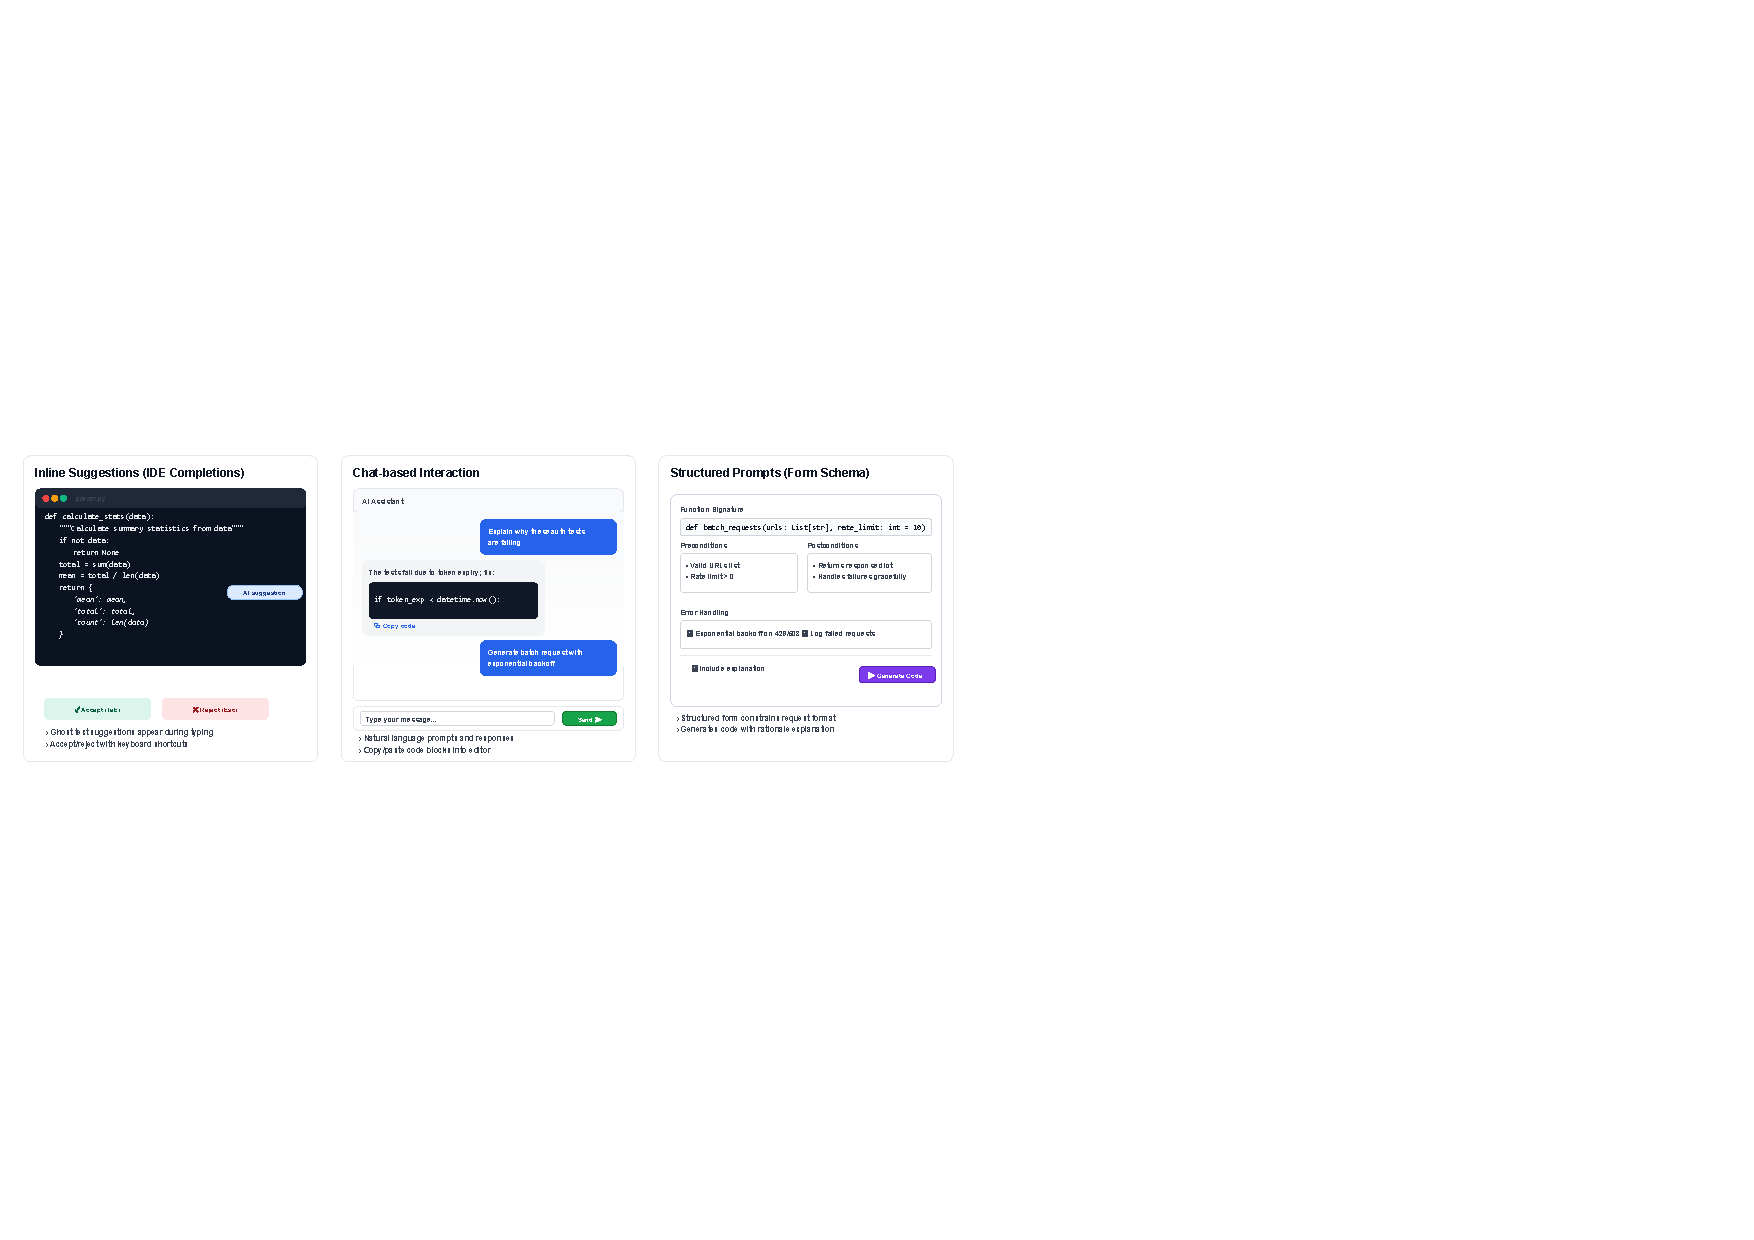
\includegraphics[width=\linewidth, keepaspectratio]{assets/interaction_modes.pdf}
\end{center}
\vspace{-2pt}
\begin{keybox}[Three Delivery Modes, One LLM]
\scriptsize
\textbf{Inline} --- ghost-text completions in the editor\\
\textbf{Chat} --- prompt/response panel with code blocks\\
\textbf{Structured} --- form schema generating code + rationale\\[2pt]
All powered by the \emph{same} GPT-4o backend with identical decoding parameters.
\end{keybox}
\end{column}
\end{columns}
\end{frame}

% ============================================================

\begin{frame}{Three Interaction Modes}
\sideAccent
\vspace{-6pt}
\begin{center}
  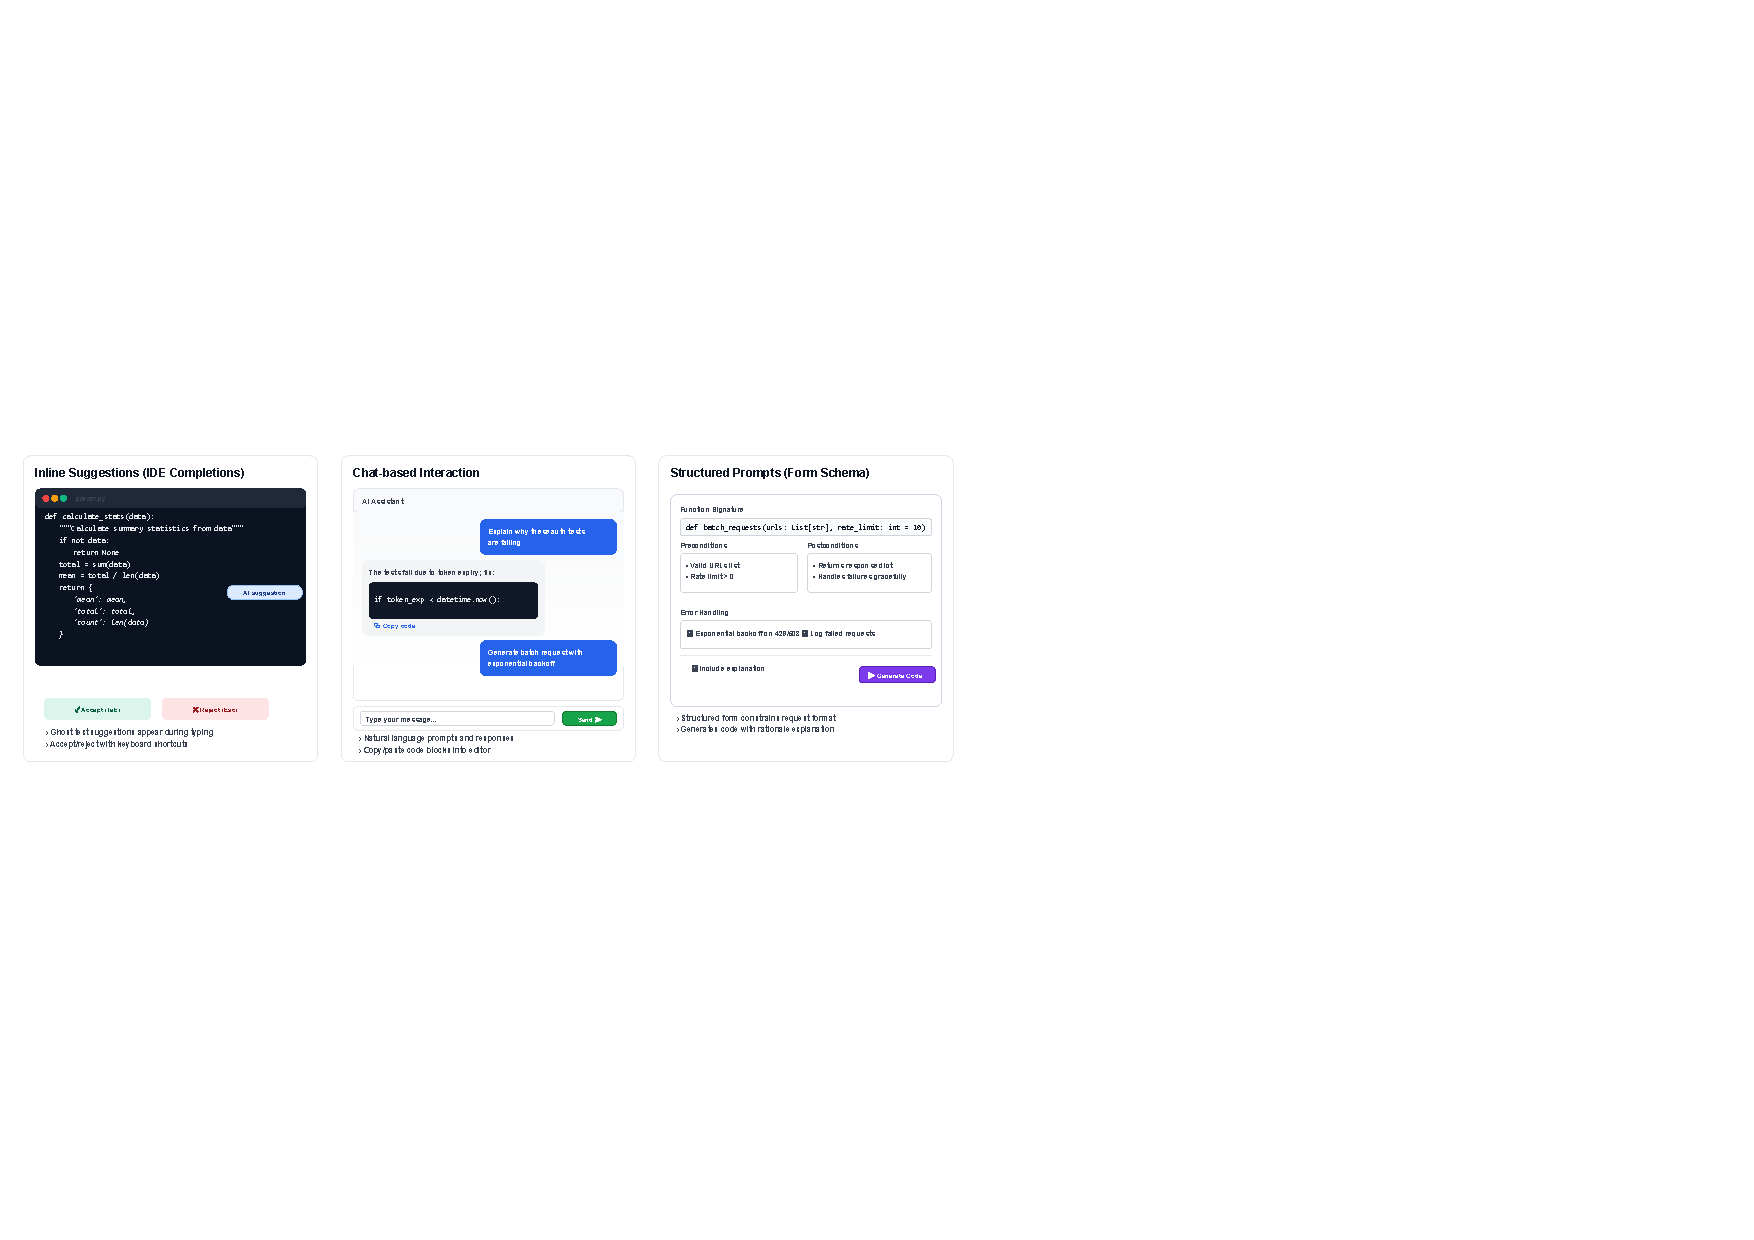
\includegraphics[width=0.82\linewidth, height=0.52\textheight, keepaspectratio]{assets/interaction_modes.pdf}
\end{center}
\vspace{-4pt}
\begin{columns}[T]
\begin{column}{0.32\textwidth}
\begin{findingbox}
\scriptsize \textbf{Inline Suggestions}\\
Ghost-text completions at syntactically stable points. Accept/partial-accept/reject via keyboard. Logged: offer, accept, edited-after-accept, reject events with timestamps.
\end{findingbox}
\end{column}
\begin{column}{0.32\textwidth}
\begin{findingbox}
\scriptsize \textbf{Chat-based Interaction}\\
Dedicated IDE panel for natural-language prompts. Copy/paste code blocks into editor. Logged: prompt turns, response lengths, code-block extractions, paste events.
\end{findingbox}
\end{column}
\begin{column}{0.32\textwidth}
\begin{findingbox}
\scriptsize \textbf{Structured Prompts}\\
Form schema: function signature, pre/post-conditions, constraints, error handling, test hints. Generates code + 1-paragraph rationale. Logged: field values \& generation events.
\end{findingbox}
\end{column}
\end{columns}
\end{frame}

% ============================================================

\begin{frame}{Gaps \& Research Questions}
\sideAccent
\vspace{2pt}
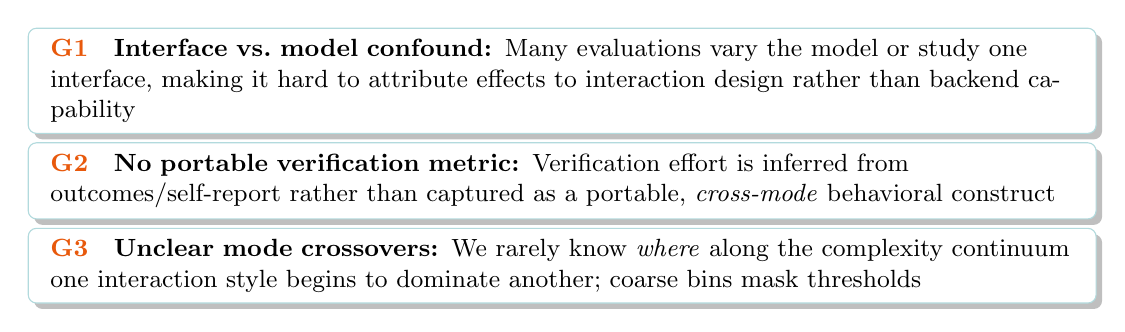
\begin{tikzpicture}[
  gap/.style={rounded corners=3pt, fill=white, draw=chiTeal!30,
    text width=13cm, align=left, font=\small,
    inner xsep=8pt, inner ysep=4pt, drop shadow}]
  \node[gap] (g1) at (0,0) {
    \textcolor{chiAccent}{\textbf{G1}} ~~\textbf{Interface vs.\ model confound:} Many evaluations vary the model or study one interface, making it hard to attribute effects to interaction design rather than backend capability};
  \node[gap, below=3pt of g1] (g2) {
    \textcolor{chiAccent}{\textbf{G2}} ~~\textbf{No portable verification metric:} Verification effort is inferred from outcomes/self-report rather than captured as a portable, \emph{cross-mode} behavioral construct};
  \node[gap, below=3pt of g2] (g3) {
    \textcolor{chiAccent}{\textbf{G3}} ~~\textbf{Unclear mode crossovers:} We rarely know \emph{where} along the complexity continuum one interaction style begins to dominate another; coarse bins mask thresholds};
\end{tikzpicture}

\vspace{4pt}
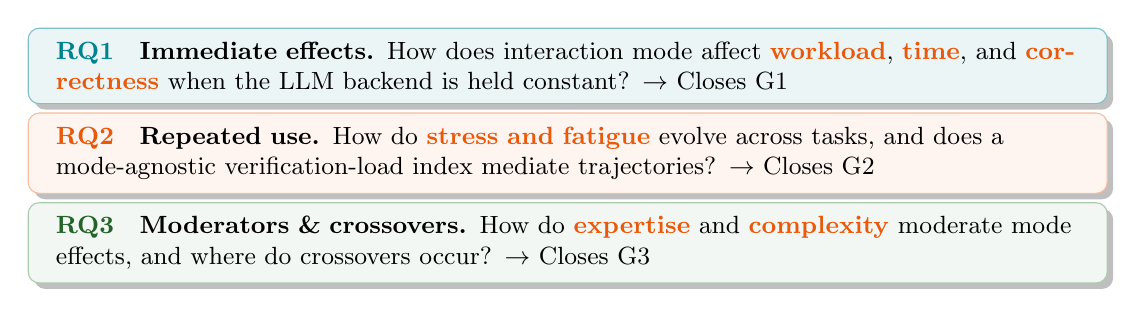
\begin{tikzpicture}[
  rq/.style={rounded corners=4pt, text width=13cm, align=left, font=\small,
    inner xsep=10pt, inner ysep=5pt, drop shadow}]
  \node[rq, fill=chiTeal!8, draw=chiTeal!50] (r1) at (0,0) {
    \textcolor{chiTeal}{\textbf{RQ1}} ~~\textbf{Immediate effects.} How does interaction mode affect \emphmark{workload}, \emphmark{time}, and \emphmark{correctness} when the LLM backend is held constant? $\to$ Closes G1};
  \node[rq, fill=chiAccent!6, draw=chiAccent!40, below=3pt of r1] (r2) {
    \textcolor{chiAccent}{\textbf{RQ2}} ~~\textbf{Repeated use.} How do \emphmark{stress and fatigue} evolve across tasks, and does a mode-agnostic verification-load index mediate trajectories? $\to$ Closes G2};
  \node[rq, fill=chiGreen!6, draw=chiGreen!40, below=3pt of r2] (r3) {
    \textcolor{chiGreen!80!black}{\textbf{RQ3}} ~~\textbf{Moderators \& crossovers.} How do \emphmark{expertise} and \emphmark{complexity} moderate mode effects, and where do crossovers occur? $\to$ Closes G3};
\end{tikzpicture}
\end{frame}

% ============================================================
%  SECTION 2: STUDY DESIGN
% ============================================================
{
\setbeamertemplate{footline}{}
\begin{frame}[plain,noframenumbering]
\begin{tikzpicture}[remember picture, overlay]
  \fill[chiTeal] (current page.north west) rectangle
    ([yshift=-3.5cm]current page.north east);
  \mosaicCorner{-6}{1.5}{1.5}
  \mosaicCorner{5.5}{1.0}{1.2}
  \node[anchor=west, text=white, font=\huge\bfseries]
    at ([xshift=16mm, yshift=-1.75cm]current page.north west) {2};
  \node[anchor=west, text=white, font=\Large]
    at ([xshift=28mm, yshift=-1.75cm]current page.north west)
    {Study Design};
  \draw[chiAccent, line width=2pt]
    ([xshift=16mm, yshift=-2.8cm]current page.north west) --
    ([xshift=70mm, yshift=-2.8cm]current page.north west);
  \node[anchor=north west, text=chiGray, font=\small\itshape, text width=12cm]
    at ([xshift=16mm, yshift=-4.2cm]current page.north west)
    {Counterbalanced within-subjects ($N{=}60$) with matched no-AI control};
  \node[rounded corners=3pt, fill=chiAccent, text=white, font=\small\bfseries,
    inner xsep=10pt, inner ysep=4pt]
    at ([xshift=-25mm, yshift=-1.75cm]current page.north east) {$N{=}60$};
\end{tikzpicture}
\end{frame}
}

% ============================================================

\begin{frame}{Study Design Overview}
\begin{center}
  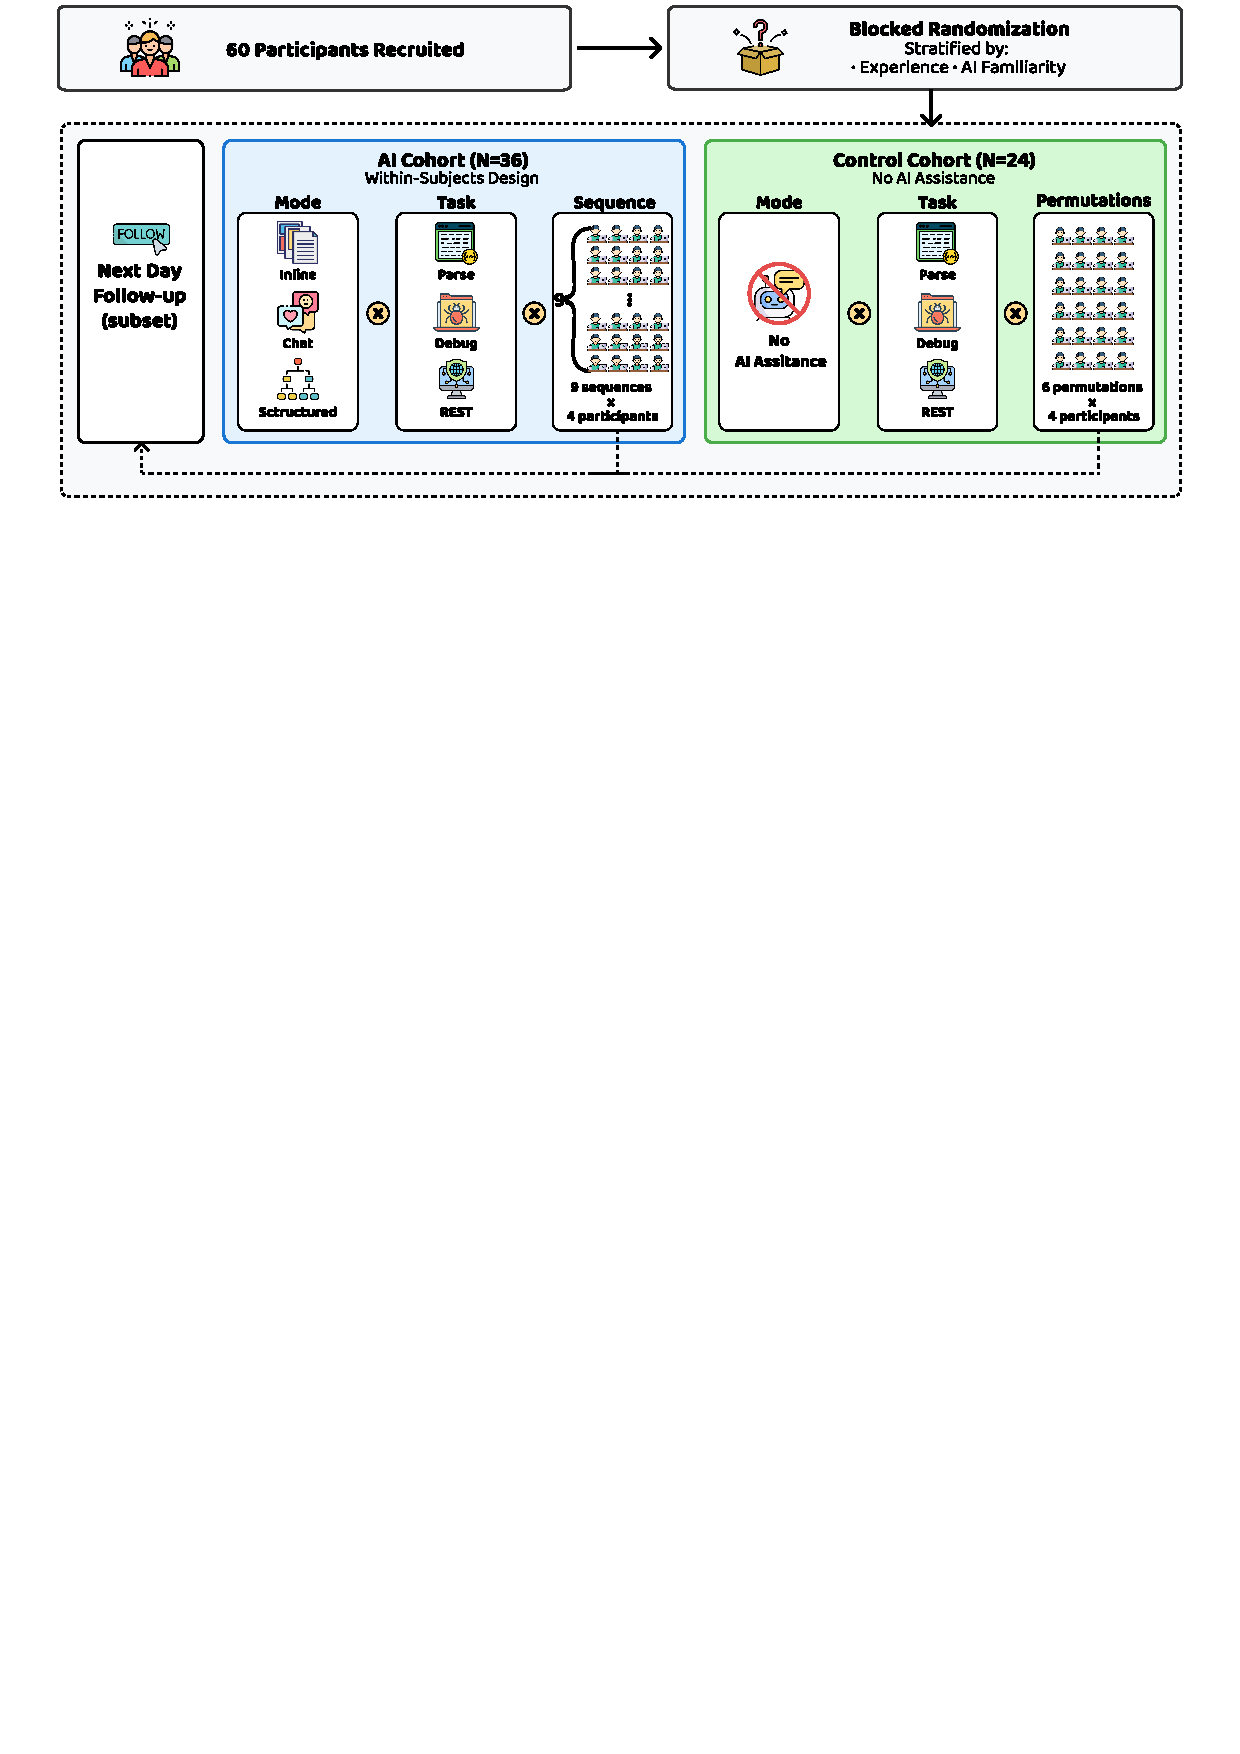
\includegraphics[width=0.6\linewidth, height=0.5\textheight, keepaspectratio]{assets/design.pdf}
\end{center}
\vspace{-2pt}
\begin{columns}[T]
\begin{column}{0.5\textwidth}
\begin{keybox}[Design Components]
\scriptsize
\textbf{D1. Within-subjects (AI, $n{=}36$):}
Each participant completed 3~tasks, one per mode, in counterbalanced order.\\[3pt]
\textbf{D2. Between-subjects Control ($n{=}24$):}
Same 3~tasks without AI, balanced task order.\\[3pt]
\textbf{D3. Next-day follow-up:}
Exploratory subset repeated a matched-complexity task.
\end{keybox}
\end{column}
\begin{column}{0.48\textwidth}
\begin{alertbox}[Counterbalancing]
\scriptsize
\textbf{9 decoupled} Task$\times$Mode sequences, \textbf{4 participants} per sequence $=$ 36 AI participants.
All $3{\times}3{=}9$ pairings occur \textbf{equally} (12 obs/cell). Each Mode appears equally at each Index (1--3). Control: 6 task-order permutations $\times$ 4.\\[2pt]
Fisher's exact: no association with experience ($p{=}0.88$).
\end{alertbox}
\end{column}
\end{columns}
\end{frame}

% ============================================================

\begin{frame}{Participants \& Tasks}
\begin{columns}[T]
\begin{column}{0.48\textwidth}
\begin{keybox}[Participant Profile ($N{=}60$)]
\scriptsize
\renewcommand{\arraystretch}{1.15}
\begin{tabular}{lccr}
\toprule
\textbf{Bin} & \textbf{AI} & \textbf{Ctrl} & \textbf{Total} \\
\midrule
Novice (2--3\,yr) & 12 & 8 & 20 \\
Intermediate (3--6\,yr) & 16 & 12 & 28 \\
Experienced ($\geq$6\,yr) & 8 & 4 & 12 \\
\midrule
\textbf{Total} & \textbf{36} & \textbf{24} & \textbf{60} \\
\bottomrule
\end{tabular}
\vspace{3pt}

\textbf{AI tool familiarity} (weekly/daily):\\
ChatGPT 78\% \textbullet{} Copilot 62\% \textbullet{} CodeWhisperer 18\%\\[2pt]
\textbf{Languages:} Python (all), JS/TS (48\%), Java (35\%)\\
\textbf{Baseline:} Cohorts equivalent on age ($27.4{\pm}3.1$ vs $27.1{\pm}3.2$), years coding, KSS, SSSQ (all SMD $< 0.20$).
\end{keybox}
\end{column}
\begin{column}{0.50\textwidth}
\begin{alertbox}[Three Python Tasks]
\scriptsize
\renewcommand{\arraystretch}{1.15}
\begin{tabular}{p{0.22\linewidth}p{0.70\linewidth}}
\toprule
\textbf{Task} & \textbf{Description \& Complexity} \\
\midrule
\textbf{A: Parse} & CSV/JSON parser with schema validation. LOC$\approx$200, median cyclomatic $\tilde{v}{\in}[3,5]$. \textit{Low.} \\
\midrule
\textbf{B: Debug Auth} & Fix auth module (hashing, token expiry, clock skew). LOC$\approx$260, $\tilde{v}{\in}[4,6]$. \textit{Moderate.} \\
\midrule
\textbf{C: Batch REST} & REST client with rate limiting, exponential backoff, partial failure. LOC$\approx$300, $\tilde{v}{\in}[5,7]$. \textit{High.} \\
\bottomrule
\end{tabular}
\vspace{3pt}

\textbf{Oracles:} 10--12 unit tests/task (pytest), $\geq$80\% line coverage, $\geq$60\% mutation score.
40\,min cap per task; 15--20\,min breaks between tasks.
\end{alertbox}
\end{column}
\end{columns}
\end{frame}

% ============================================================

\begin{frame}{Measures \& Verification-Load Index}
\begin{columns}[T]
\begin{column}{0.52\textwidth}
\begin{center}
  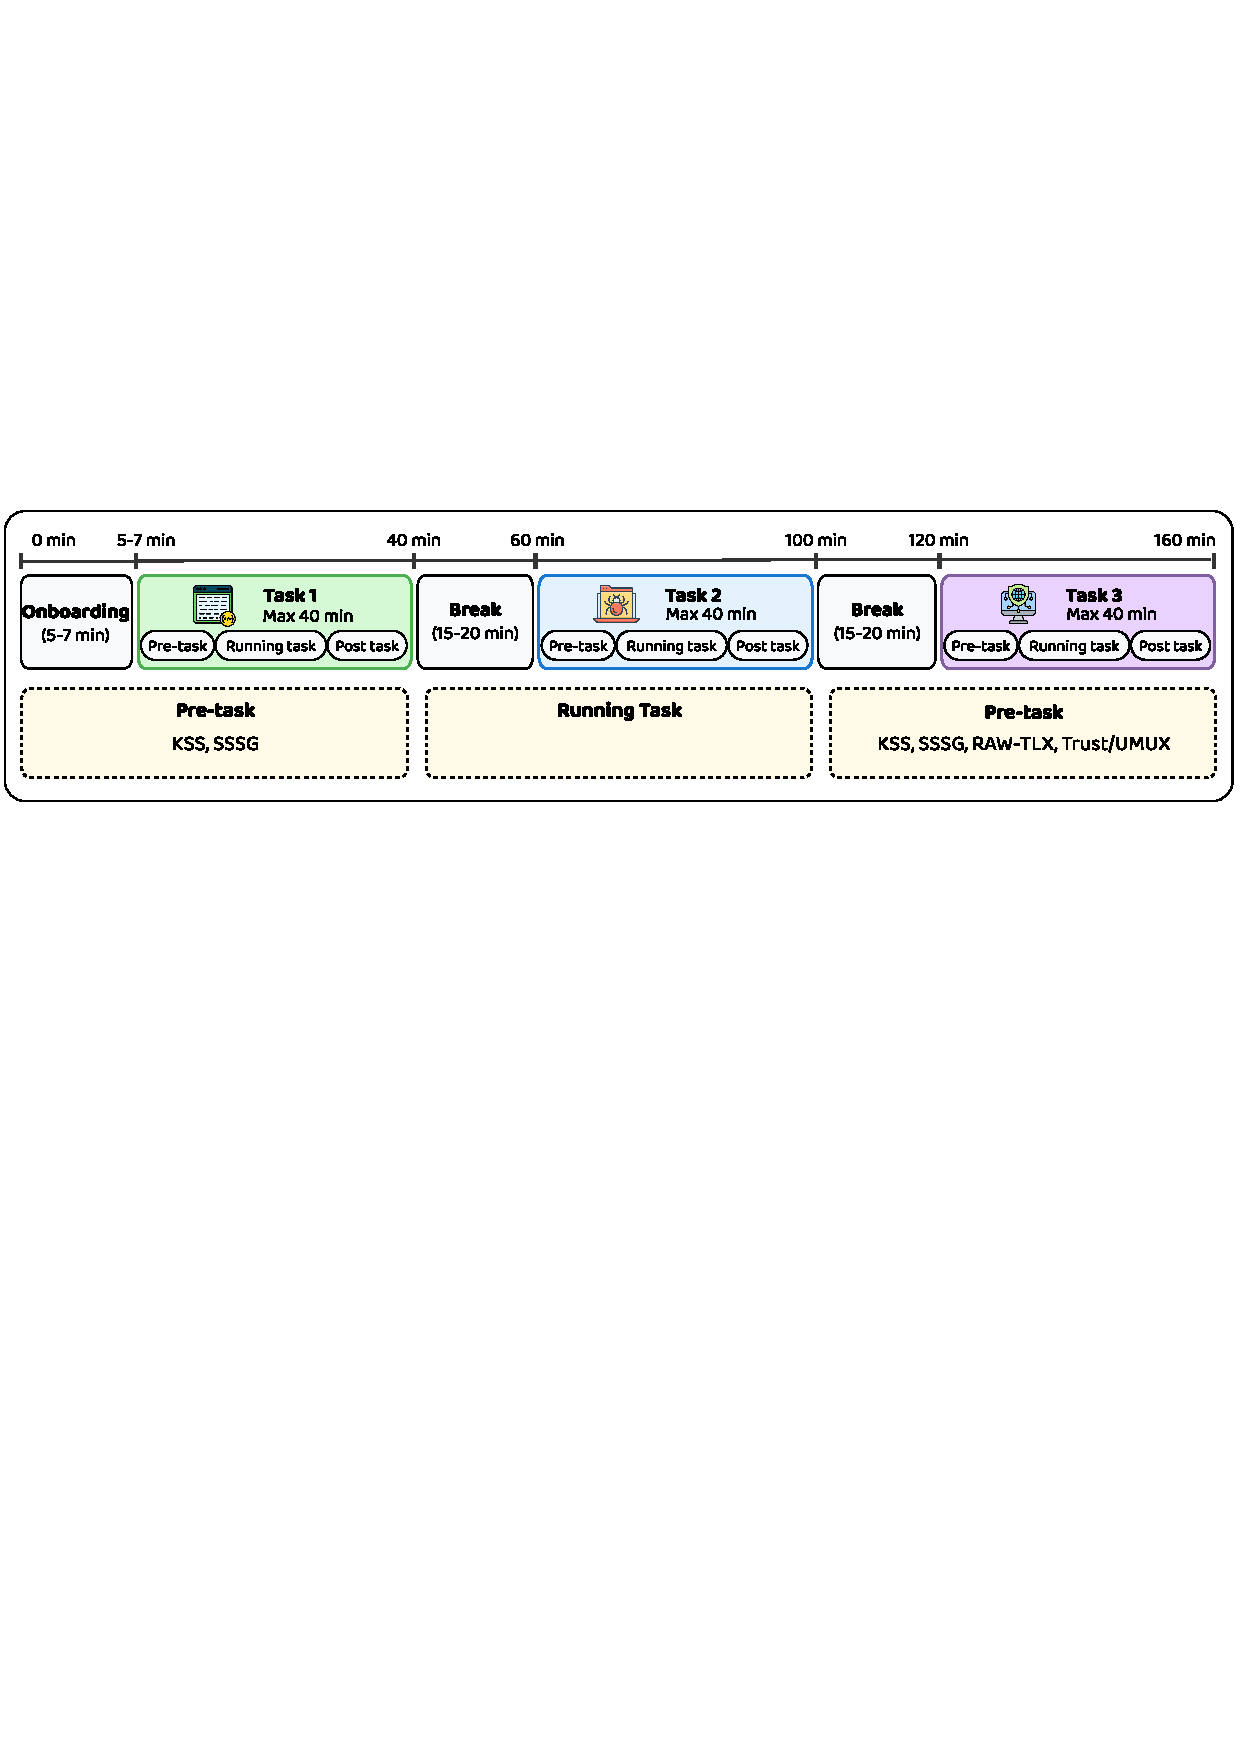
\includegraphics[width=\linewidth, height=0.58\textheight, keepaspectratio]{assets/measure.pdf}
\end{center}
\vspace{-2pt}
\begin{findingbox}
\scriptsize
\textbf{Reliability:} TLX $\alpha{=}0.86$, SSSQ $\alpha{=}0.81$, KSS test--retest $r{=}0.72$,
$V_{\text{core}}$ $\alpha{=}0.80$. Logging coverage $>$99\%; missingness $<$2\%.
\end{findingbox}
\end{column}
\begin{column}{0.46\textwidth}
\begin{keybox}[$V_{\text{core}}$: Verification-Load Composite]
\scriptsize
Mean $z$-score across \textbf{five} uniformly-logged behavioral signals:\\[3pt]
\begin{tabular}{cl}
\faExclamationTriangle & Compile/test \textbf{failures} ($\beta_{\text{KSS}}{=}0.26$)\\
\faClock & \textbf{Time-to-first-compile} ($\beta{=}0.22$)\\
\faCodeBranch & Normalized \textbf{code churn} ($\beta{=}0.12$)\\
\faPause & Cumulative \textbf{pauses} $>$2\,s ($\beta{=}0.19$)\\
\faRandom & \textbf{Context switches} ($\beta{=}0.15$)\\
\end{tabular}
\\[4pt]
PCA: dominant factor eigenvalue $=2.61$ (52.2\% variance), loadings $\geq 0.63$ for failures, time-to-first-compile, and pauses.
\end{keybox}
\vspace{1pt}
\begin{contextbox}[Other Measures]
\scriptsize
\textbf{Workload:} RAW NASA-TLX (0--100)\\
\textbf{Time:} Minutes to first full-pass (log-scale)\\
\textbf{Correctness:} Tests passed / $N$ (binomial GLMM)\\
\textbf{Fatigue:} KSS 1--9, pre \& post each task\\
\textbf{Stress:} SSSQ composite ($z$-scores)
\end{contextbox}
\end{column}
\end{columns}
\end{frame}

% ============================================================
%  SECTION 3: RQ1
% ============================================================
{
\setbeamertemplate{footline}{}
\begin{frame}[plain,noframenumbering]
\begin{tikzpicture}[remember picture, overlay]
  \fill[chiTeal] (current page.north west) rectangle
    ([yshift=-3.5cm]current page.north east);
  \mosaicCorner{-6}{1.5}{1.5}
  \mosaicCorner{5.5}{1.0}{1.2}
  \node[anchor=west, text=white, font=\huge\bfseries]
    at ([xshift=16mm, yshift=-1.75cm]current page.north west) {3};
  \node[anchor=west, text=white, font=\Large]
    at ([xshift=28mm, yshift=-1.75cm]current page.north west)
    {RQ1: Workload, Time \& Correctness};
  \draw[chiAccent, line width=2pt]
    ([xshift=16mm, yshift=-2.8cm]current page.north west) --
    ([xshift=70mm, yshift=-2.8cm]current page.north west);
  \node[anchor=north west, text=chiGray, font=\small\itshape, text width=12cm]
    at ([xshift=16mm, yshift=-4.2cm]current page.north west)
    {AI reduces workload by $-18.2$ TLX, time by 22\%, correctness OR$=1.71$};
\end{tikzpicture}
\end{frame}
}

% ============================================================

\begin{frame}{RQ1 --- NASA-TLX \& Completion Time}
\begin{columns}[T]
\begin{column}{0.60\textwidth}
\begin{center}
  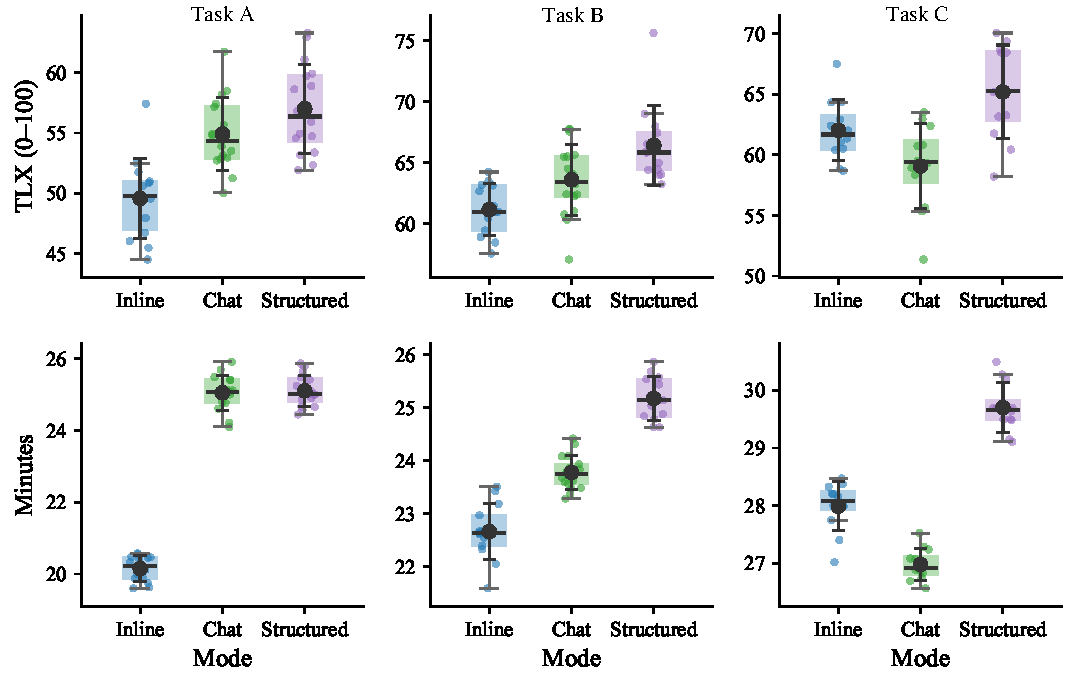
\includegraphics[width=\linewidth, height=0.72\textheight, keepaspectratio]{assets/rq1_tlx_time_combo(1).pdf}
\end{center}
\end{column}
\begin{column}{0.48\textwidth}
\begin{keybox}[AI vs.\ Control (pooled)]
\scriptsize
\textbf{Workload:} $-18.2$ TLX points\\
CI $[-22.3, -14.0]$, $p{<}0.001$\\[3pt]
\textbf{Time:} 25.0 vs 32.1\,min\\
Ratio $0.78$, CI $[0.74, 0.83]$\\
\emphmark{22\% faster}, $p{<}0.001$
\end{keybox}
\vspace{1pt}
\begin{findingbox}
\scriptsize
\textbf{Within AI --- TLX:}\\
Task A: Inline \emphmark{49.3} vs Chat 56.0 ($\Delta{=}{-}6.7$, $p{=}.006$) vs Structured 58.1 ($\Delta{=}{-}8.8$, $p{<}.001$)\\[2pt]
Task C: Chat 59.7 $\approx$ Inline 60.9 ($p{=}.48$), both $<$ Structured 66.0 ($p{=}.008$)

\textbf{Within AI --- Time:}\\
Task A: Inline \emphmark{19.9\,min} vs Chat 24.5 ($p{<}.001$) vs Structured 25.1 ($p{<}.001$)\\[2pt]
Task C: Chat 27.1 $\approx$ Inline 27.8 ($p{=}.56$), both $<$ Structured 29.7 ($p{=}.021$)
\end{findingbox}
\end{column}
\end{columns}
\end{frame}

% ============================================================

\begin{frame}{RQ1 --- Detailed Statistics}
\sideAccent
\vspace{-2pt}
\begin{center}
\scriptsize
\renewcommand{\arraystretch}{1.1}
\begin{tabular}{ll ccc}
\toprule
\textbf{Task} & \textbf{Mode} & \textbf{TLX EMM [95\% CI]} & \textbf{Time EMM (min) [95\% CI]} & \textbf{Correctness /10 [95\% CI]} \\
\midrule
A (low) & Inline     & 49.3 [45.6, 53.0] & 19.9 [18.5, 21.3] & 8.3 [8.0, 8.6] \\
        & Chat       & 56.0 [52.1, 60.0] & 24.5 [22.7, 26.4] & 8.2 [7.9, 8.5] \\
        & Structured & 58.1 [54.3, 61.9] & 25.1 [23.3, 27.0] & 8.3 [8.0, 8.6] \\
\midrule
B (mid) & Inline     & 55.4 [51.7, 59.1] & 22.5 [21.0, 24.1] & 7.2 [6.9, 7.5] \\
        & Chat       & 58.1 [54.4, 61.8] & 23.9 [22.2, 25.7] & 7.3 [7.0, 7.6] \\
        & Structured & 60.9 [57.2, 64.6] & 25.0 [23.2, 26.9] & 7.6 [7.3, 7.9] \\
\midrule
C (high)& Inline     & 60.9 [57.3, 64.6] & 27.8 [26.0, 29.8] & 7.3 [6.9, 7.7] \\
        & Chat       & 59.7 [56.1, 63.2] & 27.1 [25.4, 28.9] & \emphmark{8.0} [7.6, 8.5] \\
        & Structured & 66.0 [62.5, 69.4] & 29.7 [27.9, 31.8] & 7.1 [6.7, 7.5] \\
\bottomrule
\end{tabular}
\end{center}
\vspace{2pt}
\begin{columns}[T]
\begin{column}{0.48\textwidth}
\begin{findingbox}
\scriptsize
\textbf{Model fit --- TLX:} Mode $\chi^2(2){=}30.7$, $p{<}.001$; Mode$\times$Task $\chi^2(4){=}12.9$, $p{=}.011$. Random intercepts for participant \& task version; random slopes for Index.
\end{findingbox}
\end{column}
\begin{column}{0.48\textwidth}
\begin{findingbox}
\scriptsize
\textbf{Model fit --- Time:} Mode $\chi^2(2){=}27.6$, $p{<}.001$; Mode$\times$Task $\chi^2(4){=}11.1$, $p{=}.025$.
AFT survival robustness: Inline vs Structured HR$=1.32$ [1.12, 1.56]; Chat vs Structured HR$=1.17$ [1.00, 1.37].
\end{findingbox}
\end{column}
\end{columns}
\end{frame}

% ============================================================

\begin{frame}{RQ1 --- Correctness \& Acceptance}
\sideAccent
\vspace{-4pt}
\begin{columns}[T]
\begin{column}{0.58\textwidth}
\begin{center}
  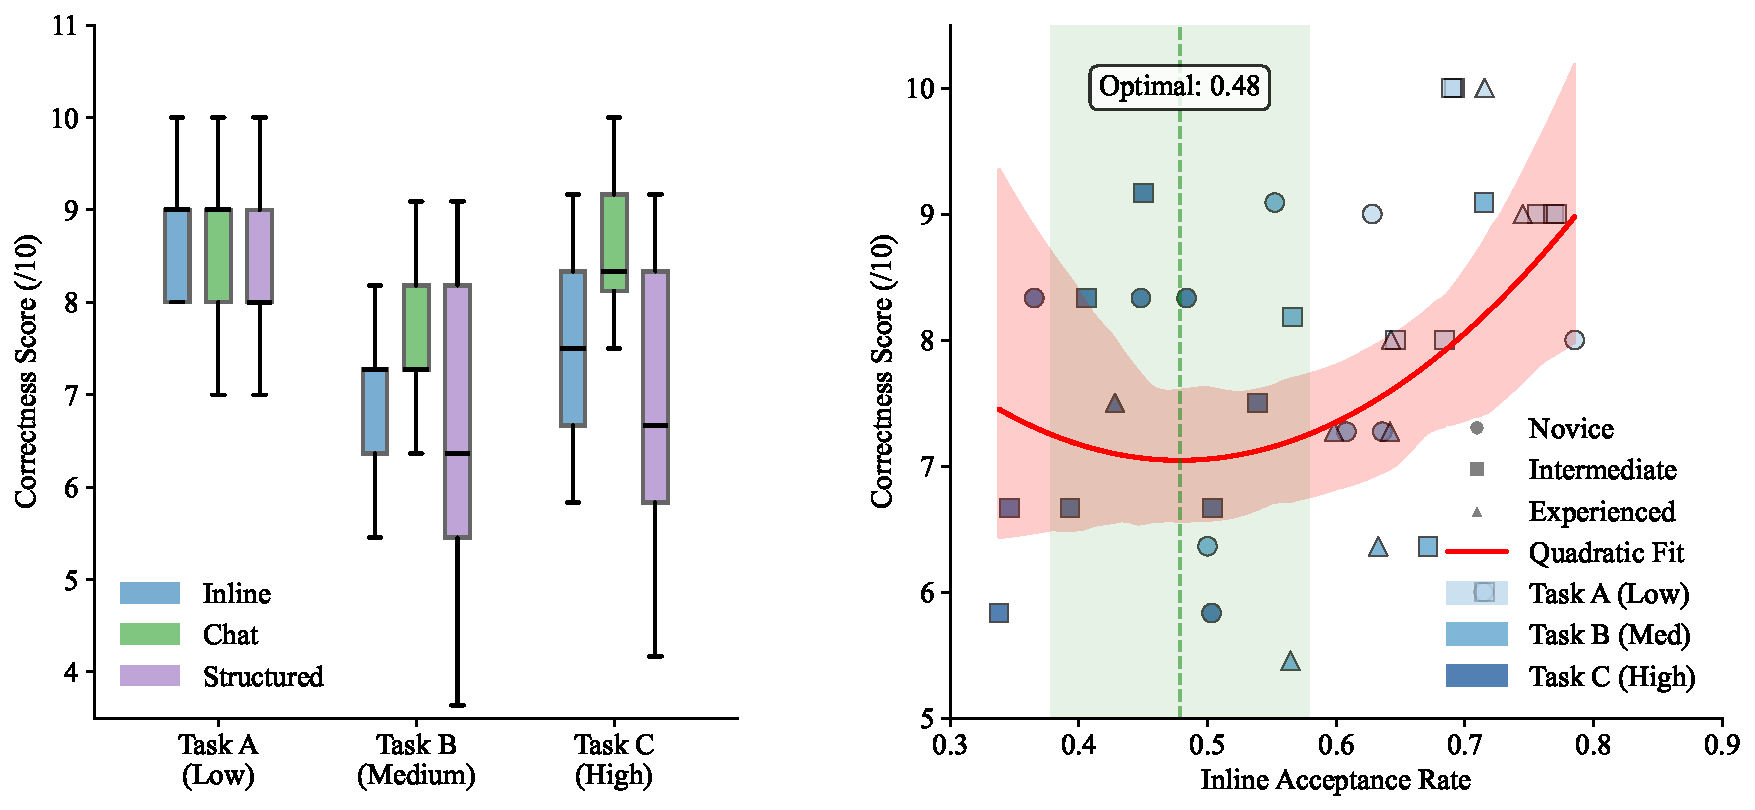
\includegraphics[width=\linewidth, height=0.72\textheight, keepaspectratio]{assets/figure2_correctness.pdf}
\end{center}
\begin{keybox}[AI vs.\ Control --- Correctness]
\scriptsize
AI EMM $=7.6/10$, Control $=6.2/10$\\
OR $= \mathbf{1.71}$, CI $[1.37, 2.13]$, $p{<}.001$\\[2pt]
GLMM: Mode$\times$Task $\chi^2(4){=}12.1$, $p{=}.016$
\end{keybox}
\end{column}
\begin{column}{0.40\textwidth}
\begin{findingbox}
\scriptsize
\textbf{Task C (high complexity):}\\
Chat \emphmark{8.0}/10 vs Inline 7.3 ($p{=}.009$) vs Structured 7.1 ($p{=}.005$).\\[3pt]
\textbf{Task B (moderate):}\\
Structured 7.6 vs Inline 7.2 ($p{=}.041$).\\[3pt]
\textbf{Task A (low):}\\
All modes $\approx$ 8.3/10 ($p{>}.10$).
\end{findingbox}
\vspace{3pt}
\begin{alertbox}[Acceptance Sweet Spot]
\scriptsize
Inline acceptance rate vs.\ correctness follows a \textbf{quadratic} curve (Wald $p{=}.005$).
Optimum at $\hat{p}{\approx}\mathbf{0.48}$, CI $[0.44, 0.53]$.
Blind acceptance \emph{and} near-total rejection both hurt outcomes.
\end{alertbox}
\end{column}
\end{columns}
\end{frame}

% ============================================================
%  SECTION 4: RQ2
% ============================================================
{
\setbeamertemplate{footline}{}
\begin{frame}[plain,noframenumbering]
\begin{tikzpicture}[remember picture, overlay]
  \fill[chiTeal] (current page.north west) rectangle
    ([yshift=-3.5cm]current page.north east);
  \mosaicCorner{-6}{1.5}{1.5}
  \mosaicCorner{5.5}{1.0}{1.2}
  \node[anchor=west, text=white, font=\huge\bfseries]
    at ([xshift=16mm, yshift=-1.75cm]current page.north west) {4};
  \node[anchor=west, text=white, font=\Large]
    at ([xshift=28mm, yshift=-1.75cm]current page.north west)
    {RQ2: Fatigue, Stress \& Mediation};
  \draw[chiAccent, line width=2pt]
    ([xshift=16mm, yshift=-2.8cm]current page.north west) --
    ([xshift=70mm, yshift=-2.8cm]current page.north west);
  \node[anchor=north west, text=chiGray, font=\small\itshape, text width=12cm]
    at ([xshift=16mm, yshift=-4.2cm]current page.north west)
    {Verification load accounts for $\sim$26\% of rising fatigue across tasks};
\end{tikzpicture}
\end{frame}
}

% ============================================================

\begin{frame}{RQ2 --- Fatigue \& Stress Trajectories}
\begin{columns}[T]
\begin{column}{0.56\textwidth}
\begin{center}
  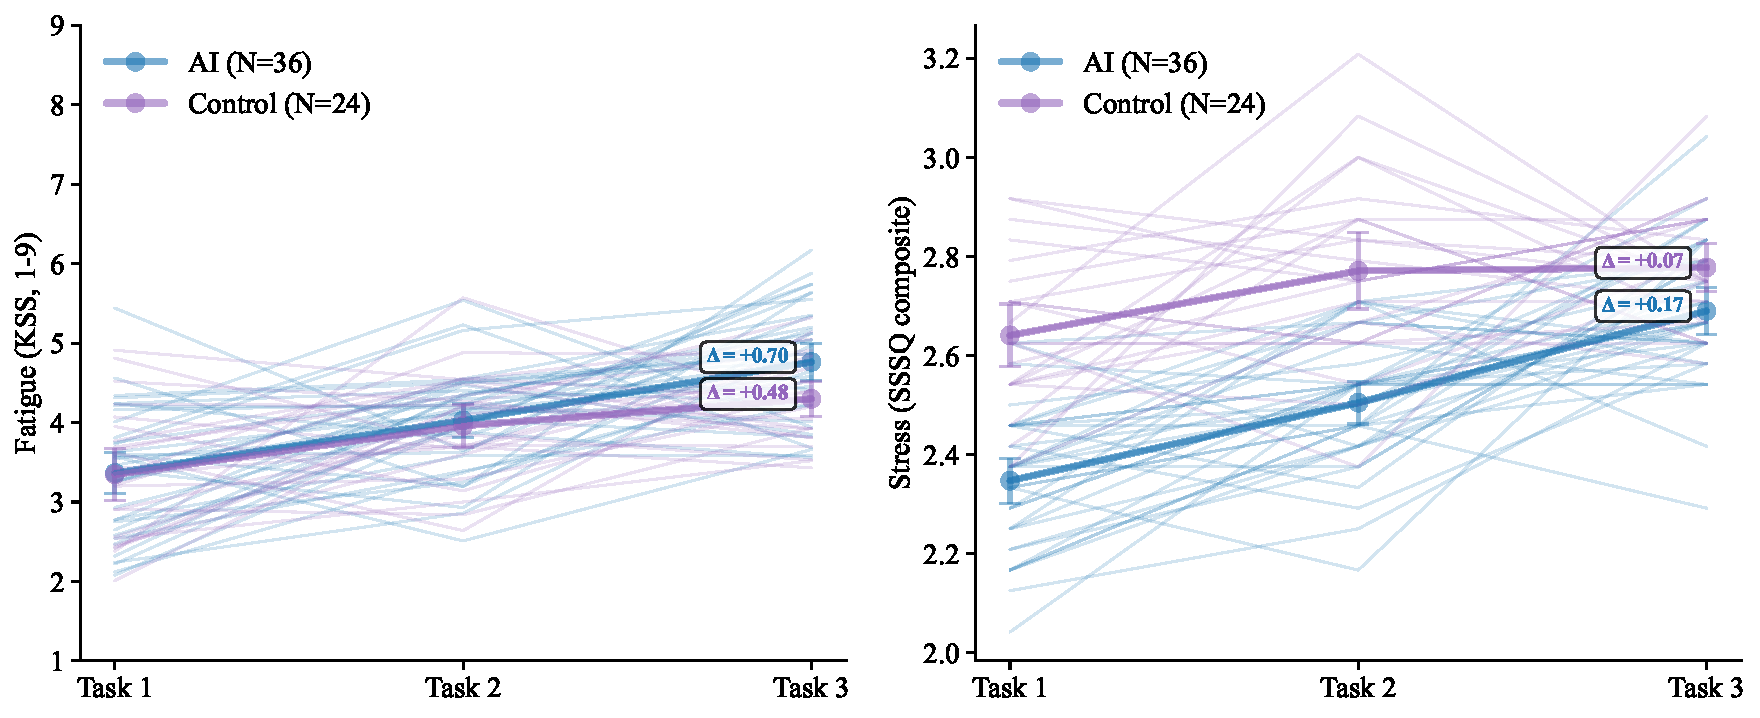
\includegraphics[width=\linewidth, height=0.70\textheight, keepaspectratio]{assets/figure3_trajectories.pdf}
\end{center}
\end{column}
\begin{column}{0.42\textwidth}
\begin{keybox}[Trajectory Slopes (Task 1 $\to$ 3)]
\scriptsize
\renewcommand{\arraystretch}{1.2}
\begin{tabular}{lcc}
\toprule
 & \textbf{KSS $\Delta$} & \textbf{SSSQ $\Delta$ ($z$)} \\
\midrule
\textbf{AI}      & \emphmark{+0.70} & +0.17 \\
                  & {\scriptsize [0.48, 0.92]} & {\scriptsize [0.06, 0.28]} \\
\textbf{Control} & +0.48 & +0.07 \\
                  & {\scriptsize [0.28, 0.68]} & {\scriptsize [$-$0.01, 0.15]} \\
\midrule
$p$ (Cond$\times$Idx) & 0.041 & 0.110 \\
\bottomrule
\end{tabular}
\end{keybox}
\vspace{1pt}
\begin{findingbox}
\scriptsize
\textbf{Per-mode slopes (KSS within AI):}\\
Inline $\Delta{=}$\emphmark{+1.18} (steepest)\\
Structured $\Delta{=}+1.05$\\
Chat $\Delta{=}+0.92$ (shallowest)\\[2pt]
Mode$\times$Index: $\chi^2(2){=}6.8$, $p{=}.033$\\
Inline--Chat $\Delta{=}0.26$, $p{=}.048$
\end{findingbox}
\end{column}
\end{columns}
\end{frame}

% ============================================================

\begin{frame}{RQ2 --- $V_{\text{core}}$ Mediation Path Diagram}
\sideAccent
\vspace{-2pt}
\begin{center}
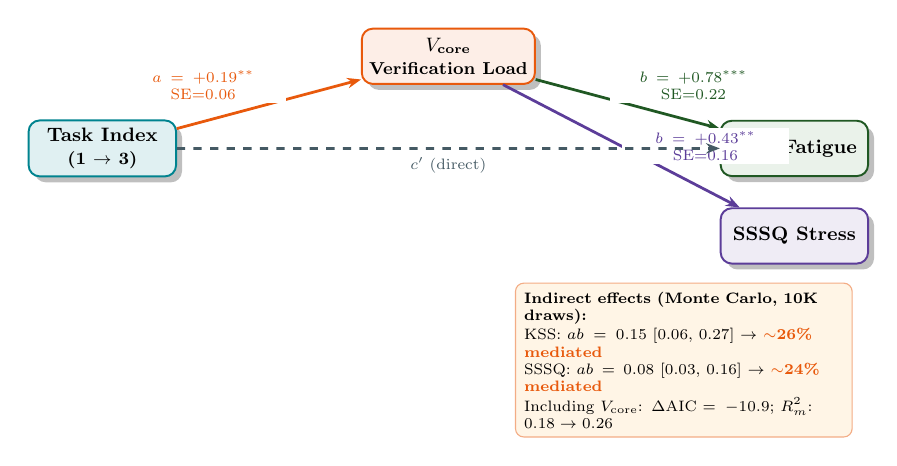
\begin{tikzpicture}[
  scale=0.78, every node/.style={transform shape},
  box/.style={rounded corners=4pt, minimum width=2.4cm, minimum height=0.9cm,
    align=center, font=\small\bfseries, drop shadow, draw, line width=0.7pt},
  arr/.style={-{Stealth[length=5pt]}, line width=1pt},
  lbl/.style={font=\scriptsize, fill=white, inner sep=1.5pt, align=center, text width=2.6cm},
  node distance=3cm
]
  % Nodes
  \node[box, fill=chiTeal!12, draw=chiTeal] (X) {Task Index\\{\footnotesize (1 $\to$ 3)}};
  \node[box, fill=chiAccent!10, draw=chiAccent, right=3cm of X, yshift=1.5cm] (M) {$V_{\text{core}}$\\{\footnotesize Verification Load}};
  \node[box, fill=chiGreen!10, draw=chiGreen!70!black, right=3cm of M, yshift=-1.5cm] (Y1) {KSS Fatigue};
  \node[box, fill=chiPurple!10, draw=chiPurple, below=0.5cm of Y1] (Y2) {SSSQ Stress};

  % Paths
  \draw[arr, chiAccent] (X) -- node[lbl, above left, xshift=3mm] {$a = +0.19^{**}$\\{\scriptsize SE$=$0.06}} (M);
  \draw[arr, chiGreen!70!black] (M) -- node[lbl, above right, xshift=-3mm] {$b = +0.78^{***}$\\{\scriptsize SE$=$0.22}} (Y1);
  \draw[arr, chiPurple] (M) -- node[lbl, right] {$b = +0.43^{**}$\\{\scriptsize SE$=$0.16}} (Y2);
  \draw[arr, chiGray, dashed] (X) -- node[lbl, below, yshift=-2pt] {$c'$ (direct)} (Y1);

  % Indirect effects box
  \node[rounded corners=3pt, fill=chiWarm!80, draw=chiAccent!50,
    text width=5.2cm, align=left, font=\scriptsize, inner sep=4pt,
    below=0.3cm of Y2, xshift=-1.8cm] (ind) {
    \textbf{Indirect effects (Monte Carlo, 10K draws):}\\[1pt]
    KSS: $ab = 0.15$ [0.06, 0.27] $\to$ \emphmark{$\sim$26\% mediated}\\
    SSSQ: $ab = 0.08$ [0.03, 0.16] $\to$ \emphmark{$\sim$24\% mediated}\\[1pt]
    Including $V_{\text{core}}$: $\Delta$AIC $= -10.9$; $R^2_m$: $0.18 \to 0.26$
  };
\end{tikzpicture}
\end{center}
\vspace{1pt}
\begin{findingbox}
\scriptsize
\textbf{Interpretation:} Verification load---the behavioral cost of checking/repairing AI output---\emph{partially mediates} rising fatigue and stress across tasks. Checking/repairing, not generation per se, is a substantive driver of repeated-use burden.
Sensitivity check with extended $V_{\text{plus}}$: KSS $ab{=}0.19$ [0.08, 0.32], SSSQ $ab{=}0.11$ [0.04, 0.20]---conclusions unchanged.
\end{findingbox}
\end{frame}

% ============================================================
%  SECTION 5: RQ3
% ============================================================
{
\setbeamertemplate{footline}{}
\begin{frame}[plain,noframenumbering]
\begin{tikzpicture}[remember picture, overlay]
  \fill[chiTeal] (current page.north west) rectangle
    ([yshift=-3.5cm]current page.north east);
  \mosaicCorner{-6}{1.5}{1.5}
  \mosaicCorner{5.5}{1.0}{1.2}
  \node[anchor=west, text=white, font=\huge\bfseries]
    at ([xshift=16mm, yshift=-1.75cm]current page.north west) {5};
  \node[anchor=west, text=white, font=\Large]
    at ([xshift=28mm, yshift=-1.75cm]current page.north west)
    {RQ3: Expertise \& Complexity Crossovers};
  \draw[chiAccent, line width=2pt]
    ([xshift=16mm, yshift=-2.8cm]current page.north west) --
    ([xshift=70mm, yshift=-2.8cm]current page.north west);
  \node[anchor=north west, text=chiGray, font=\small\itshape, text width=12cm]
    at ([xshift=16mm, yshift=-4.2cm]current page.north west)
    {Chat surpasses Inline in correctness at $z \approx +0.41$ complexity};
\end{tikzpicture}
\end{frame}
}

% ============================================================

\begin{frame}{RQ3 --- Expertise Moderation}
\begin{columns}[T]
\begin{column}{0.56\textwidth}
\begin{center}
  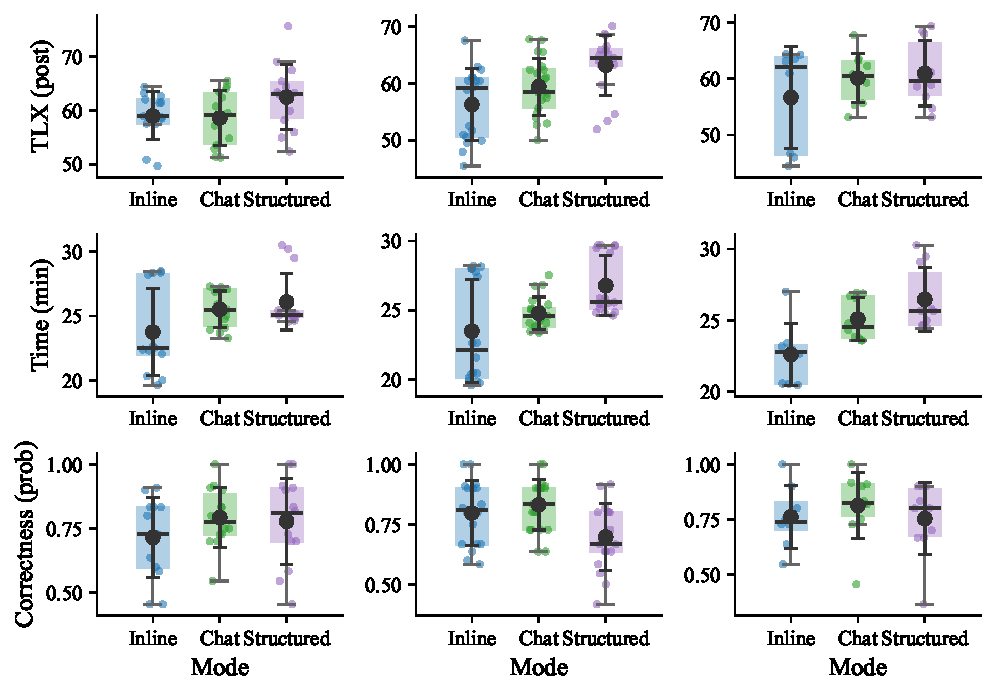
\includegraphics[width=\linewidth, height=0.6\textheight, keepaspectratio]{assets/rq3_expertise_facets(1).pdf}
\end{center}
\begin{findingbox}
\scriptsize
\textbf{Experienced ($n{=}8$):}
Inline minimizes TLX/time on simple ($\Delta{=}{-}8.0$ pts, $p{=}.007$; ratio $0.78$, $p{=}.004$).
On high: Chat $\uparrow$ correctness (8.4 vs 7.6, $p{=}.017$) without time penalty ($p{=}.34$).
Structured consistently most effortful ($+5.0$ TLX pts, $p{=}.031$).
\end{findingbox}
\end{column}
\begin{column}{0.42\textwidth}
\begin{keybox}[Mode $\times$ Expertise Tests]
\scriptsize
TLX: $\chi^2(4){=}10.9$, $p{=}.028$\\
Correctness: $\chi^2(4){=}9.6$, $p{=}.048$\\
Log-time: $\chi^2(4){=}8.1$, $p{=}.088$ (trend)
\end{keybox}
\vspace{1pt}
\begin{findingbox}
\scriptsize
\textbf{Novices ($n{=}12$):}
Structured $\downarrow$ TLX on mid-complexity ($\Delta{=}{-}6.2$ pts, $p{=}.012$), $\uparrow$ correctness (7.8 vs 7.1/10, OR$=$1.37, $p{=}.043$).
On high: Chat beats Inline correctness (7.7 vs 7.0, $p{=}.039$).
\end{findingbox}
\vspace{1pt}
\begin{findingbox}
\scriptsize
\textbf{Intermediate ($n{=}16$):}
Inline fastest on simple (4.5\,min advantage, $p{<}.001$); on high complexity Chat correctness edge (8.0 vs 7.5, $p{=}.091$ trend).
\end{findingbox}
\end{column}
\end{columns}
\end{frame}

% ============================================================

\begin{frame}{RQ3 --- Johnson-Neyman Crossover Thresholds}
\begin{columns}[T]
\begin{column}{0.48\textwidth}
\begin{center}
\scriptsize
\resizebox{\linewidth}{!}{%
\begin{tabular}{p{2cm} c p{3.3cm}}
\toprule
\textbf{Contrast} & \textbf{Crossover $\hat{z}$} & \textbf{J--N Region} \\
\midrule
Chat $>$ Inline & \emphmark{+0.41} {\scriptsize [+0.17, +0.64]} & $z{>}+0.40$: Chat superior \\
\midrule
Struct.\ $>$ Inline & $\approx$0.10 {\scriptsize [$-$0.05, +0.27]} & $-0.1 \leq z \leq +0.3$: Struct.\ superior \\
\midrule
Chat $>$ Struct. & +0.32 {\scriptsize [+0.12, +0.55]} & $z{>}+0.32$: Chat superior \\
\bottomrule
\end{tabular}
}
\end{center}
\vspace{4pt}
\begin{alertbox}[Acceptance Calibration]
\scriptsize
Quadratic fit: $\beta_2{=}{-}0.81$ (SE$=0.28$, $p{=}.005$)\\
Optimal acceptance rate: $\hat{p}{=}0.48$ [0.44, 0.53]\\[2pt]
Both near-blind acceptance and near-total rejection reduce correctness---a ``sweet spot'' at $\approx$50\%.
\end{alertbox}
\end{column}
\begin{column}{0.50\textwidth}
\begin{keybox}[Practical Mode Selection Guide]
\scriptsize
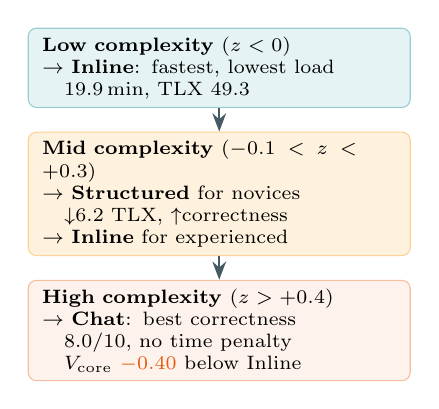
\begin{tikzpicture}[
  node distance=0.6cm,
  every node/.style={font=\scriptsize, align=left},
  box/.style={rounded corners=3pt, inner xsep=5pt, inner ysep=3pt, text width=4.5cm}
]
  \node[box, fill=chiTeal!10, draw=chiTeal!40] (low) {
    \textbf{Low complexity} ($z < 0$)\\
    $\to$ \textbf{Inline}: fastest, lowest load\\
    \quad 19.9\,min, TLX 49.3
  };
  \node[box, fill=chiYellow!15, draw=chiYellow!50, below=0.3cm of low] (mid) {
    \textbf{Mid complexity} ($-0.1 < z < +0.3$)\\
    $\to$ \textbf{Structured} for novices\\
    \quad $\downarrow$6.2 TLX, $\uparrow$correctness\\
    $\to$ \textbf{Inline} for experienced
  };
  \node[box, fill=chiAccent!8, draw=chiAccent!40, below=0.3cm of mid] (high) {
    \textbf{High complexity} ($z > +0.4$)\\
    $\to$ \textbf{Chat}: best correctness\\
    \quad 8.0/10, no time penalty\\
    \quad $V_{\text{core}}$ \emphmark{$-0.40$} below Inline
  };
  \draw[-{Stealth}, chiGray, thick] (low.south) -- (mid.north);
  \draw[-{Stealth}, chiGray, thick] (mid.south) -- (high.north);
\end{tikzpicture}
\end{keybox}
\end{column}
\end{columns}
\end{frame}

% ============================================================

\begin{frame}{RQ3 --- Verification-Load Heatmap}
\begin{columns}[T]
\begin{column}{0.58\textwidth}
\begin{center}
  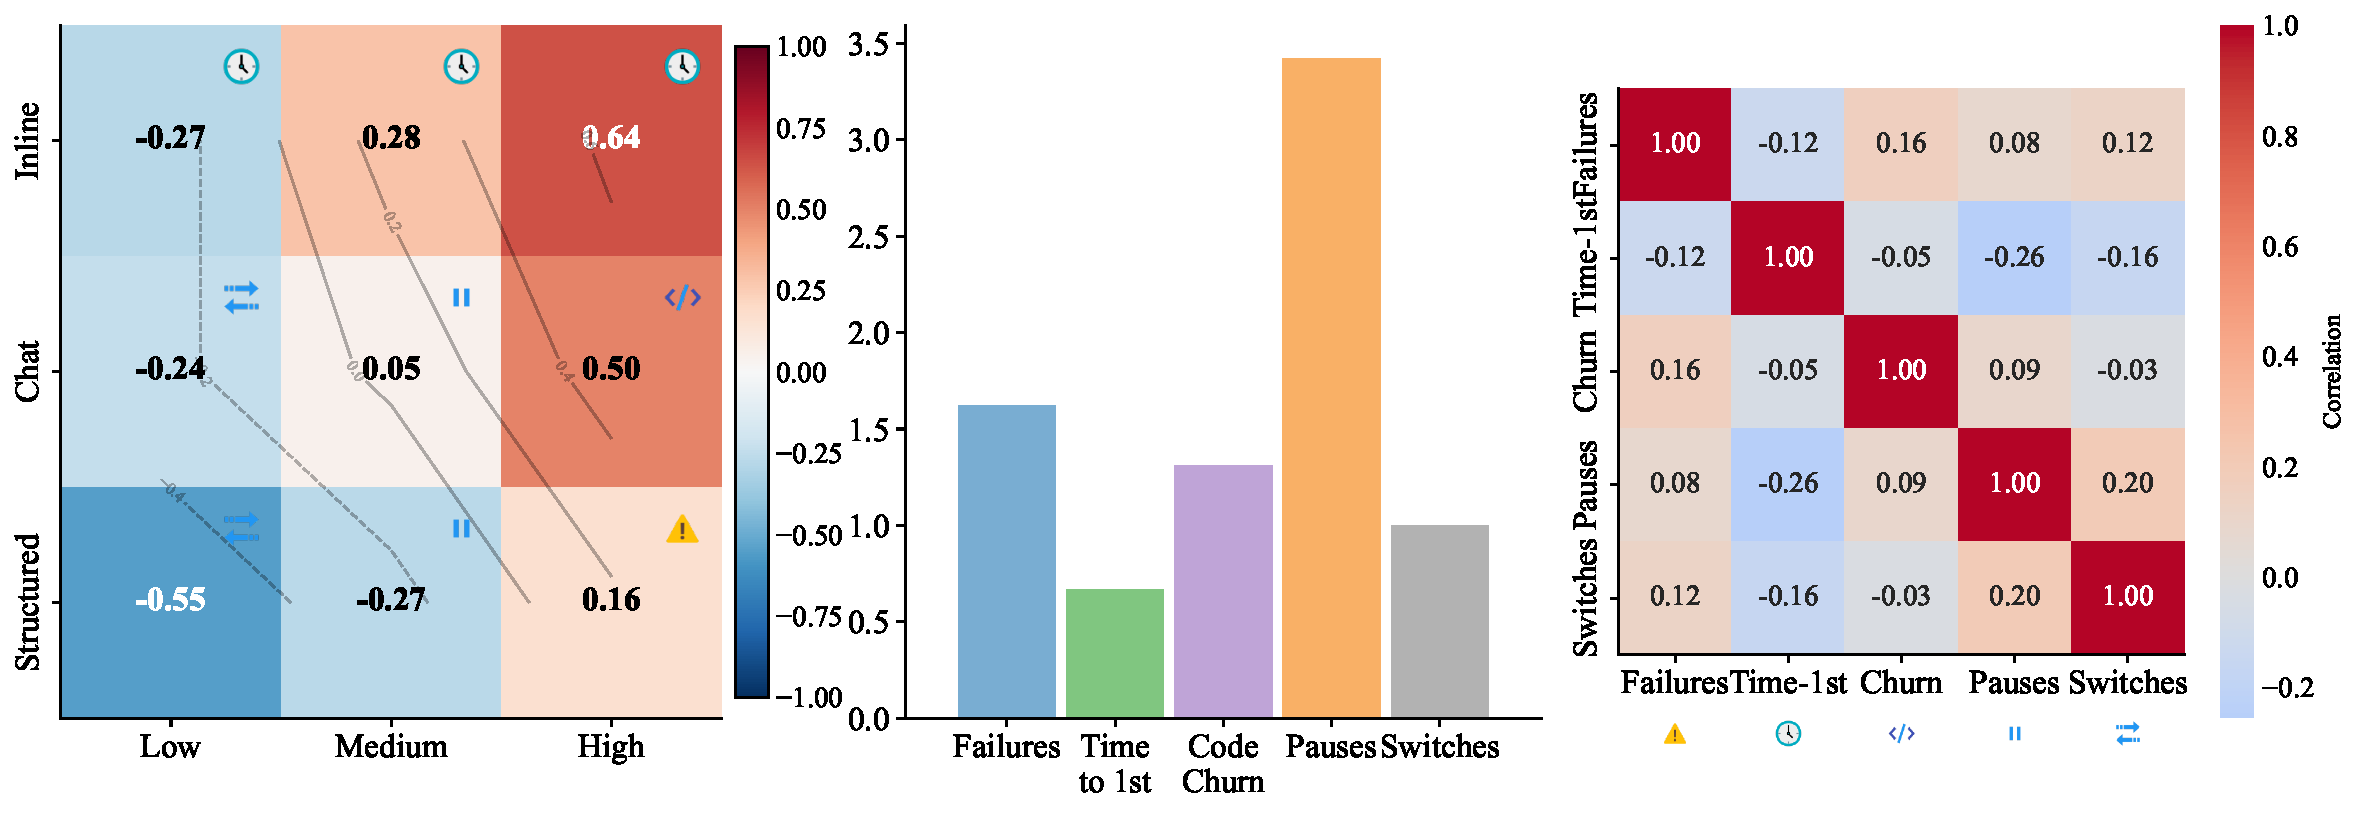
\includegraphics[width=\linewidth, height=0.72\textheight, keepaspectratio]{assets/figure10_verification_heatmap.pdf}
\end{center}
\vspace{1pt}
\begin{alertbox}[Convergent evidence]
\scriptsize
Higher $V_{\text{core}}$ $\leftrightarrow$ higher burden, lower correctness.
Chat dampens verification burden precisely when tasks are hardest.
\end{alertbox}
\end{column}
\begin{column}{0.40\textwidth}
\begin{keybox}[$V_{\text{core}}$ by Mode $\times$ Complexity]
\scriptsize
\textbf{Low complexity ($z{\approx}{-}0.6$):}\\
Inline $-0.36$ \textbullet{} Chat $-0.10$ \textbullet{} Struct.\ $+0.04$\\[3pt]
\textbf{Moderate ($z{\approx}0$):}\\
All modes converge ($p{>}.10$)\\[3pt]
\textbf{High complexity ($z{\approx}{+}0.7$):}\\
Chat \emphmark{$-0.17$} vs Inline $+0.23$ ($\Delta{=}{-}0.40$, $p{<}.001$) vs Struct.\ $+0.28$ ($\Delta{=}{-}0.45$, $p{<}.001$)
\end{keybox}
\vspace{3pt}
\begin{findingbox}
\scriptsize
\textbf{Model:} Mode $\chi^2(2){=}18.9$, $p{<}.001$;\\
Mode$\times$Complexity $\chi^2(2){=}10.6$, $p{=}.005$\\[3pt]
\textbf{Key components driving burden:}\\
Compile/test failures ($\beta{=}0.26$) and time-to-first-compile ($\beta{=}0.22$) are strongest predictors; followed by pauses ($\beta{=}0.19$) and context switches ($\beta{=}0.15$).
\end{findingbox}
\end{column}
\end{columns}
\end{frame}

% ============================================================
%  SECTION 6: DESIGN IMPLICATIONS
% ============================================================
{
\setbeamertemplate{footline}{}
\begin{frame}[plain,noframenumbering]
\begin{tikzpicture}[remember picture, overlay]
  \fill[chiTeal] (current page.north west) rectangle
    ([yshift=-3.5cm]current page.north east);
  \mosaicCorner{-6}{1.5}{1.5}
  \mosaicCorner{5.5}{1.0}{1.2}
  \node[anchor=west, text=white, font=\huge\bfseries]
    at ([xshift=16mm, yshift=-1.75cm]current page.north west) {6};
  \node[anchor=west, text=white, font=\Large]
    at ([xshift=28mm, yshift=-1.75cm]current page.north west)
    {Design Implications \& Contributions};
  \draw[chiAccent, line width=2pt]
    ([xshift=16mm, yshift=-2.8cm]current page.north west) --
    ([xshift=70mm, yshift=-2.8cm]current page.north west);
\end{tikzpicture}
\end{frame}
}

% ============================================================

\begin{frame}{Four Design Principles}
\sideAccent
\vspace{2pt}
\begin{tikzpicture}[
  dp/.style={rounded corners=3pt, text width=13.4cm, align=left, font=\small,
    inner xsep=8pt, inner ysep=4pt, drop shadow}]
  \node[dp, fill=chiTeal!7, draw=chiTeal!30] (d1) at (0,0) {
    \textcolor{chiTeal}{\faRandom~~\textbf{1.\ Adaptive Mode Orchestration}} ---
    \emph{Trigger:} $V_{\mathrm{core}}$ rising (compile failures $\uparrow$, time-to-first-compile $\uparrow$, pause clusters).
    \emph{Action:} prompt switch from Inline to Chat to reframe the problem.
    \emph{Why:} Chat dampens error cascades as complexity increases ($\Delta V_{\text{core}}{=}{-}0.40$, $p{<}.001$).};
  \node[dp, fill=chiAccent!5, draw=chiAccent!30, below=3pt of d1] (d2) {
    \textcolor{chiAccent}{\faEye~~\textbf{2.\ Transparency on Demand}} ---
    \emph{Trigger:} risky lines/diffs (predicted test failures, high-entropy edits).
    \emph{Action:} reveal micro-rationales and uncertainty at line/diff level; avoid always-on global confidences.
    \emph{Why:} on-demand cues reduce overreliance without adding constant cognitive overhead.};
  \node[dp, fill=chiGreen!5, draw=chiGreen!30, below=3pt of d2] (d3) {
    \textcolor{chiGreen!80!black}{\faClipboardList~~\textbf{3.\ Scaffolded Authoring}} ---
    \emph{Trigger:} novice profile or ambiguous requirements.
    \emph{Action:} optional Structured prompts eliciting pre/post-conditions, edge cases, I/O contracts; generate test scaffolds.
    \emph{Why:} reduces extraneous load for novices ($\Delta$TLX$={-}6.2$, correctness OR$=1.37$).};
  \node[dp, fill=chiPurple!5, draw=chiPurple!25, below=3pt of d3] (d4) {
    \textcolor{chiPurple}{\faBoxOpen~~\textbf{4.\ Verification-Aware Packaging}} ---
    \emph{Trigger:} large or multi-file edits.
    \emph{Action:} batch suggestions into testable chunks with ``try-run'' sandbox.
    \emph{Why:} lowers failure cascades and churn---the strongest contributors to burden ($\beta{=}0.26$, $0.22$).};
\end{tikzpicture}
\end{frame}

% ============================================================

\begin{frame}{Participant Voices --- Qualitative Themes}
\vspace{-3pt}
\begin{columns}[T]
\begin{column}{0.48\textwidth}
\begin{quotebox}
\scriptsize
\textbf{Theme A: Speed vs.\ Certainty}\\[3pt]
\textit{``Inline keeps me in the zone for boilerplate---I barely think about it.''}\\
\hfill{\scriptsize --- P23, Experienced, Copilot daily}\\[4pt]
\textit{``When it's gnarly, I ask Chat to lay out steps; fewer trips back and forth with tests.''}\\
\hfill{\scriptsize --- P07, Intermediate, ChatGPT weekly}
\end{quotebox}
\vspace{-3pt}
\begin{quotebox}
\scriptsize
\textbf{Theme B: Trust Shocks}\\[3pt]
\textit{``It looked right, but a missing edge case blew up tests---then I started rejecting more.''}\\
\hfill{\scriptsize --- P11, Experienced, Copilot weekly}\\[4pt]
\textit{``Two confident suggestions were wrong; I lost trust and slowed down.''}\\
\hfill{\scriptsize --- P14, Intermediate, Copilot weekly}
\end{quotebox}
\end{column}
\begin{column}{0.48\textwidth}
\begin{quotebox}
\scriptsize
\textbf{Theme C: Scaffold Me}\\[3pt]
\textit{``The form forced me to spell out inputs/outputs---I wouldn't have thought of some checks.''}\\
\hfill{\scriptsize --- P05, Novice, ChatGPT monthly}\\[4pt]
\textit{``Having constraints up front stopped me from guessing the API.''}\\
\hfill{\scriptsize --- P32, Novice, Copilot rarely}
\end{quotebox}
\vspace{-3pt}
\begin{quotebox}
\scriptsize
\textbf{Theme D: Review Fatigue}\\[3pt]
\textit{``After the fifth bad suggestion I just opened the chat and asked for a plan.''}\\
\hfill{\scriptsize --- P18, Intermediate, Copilot weekly}\\[4pt]
\textit{``Once I start rejecting a lot, it snowballs; I need a different kind of help.''}\\
\hfill{\scriptsize --- P09, Intermediate, Copilot weekly}
\end{quotebox}
\end{column}
\end{columns}
\begin{alertbox}[Behavioral Signal]
\scriptsize
Rejection streaks ($\geq$5 within 3\,min) predicted Inline$\to$Chat switches: OR$=2.36$ [1.33, 4.20], $p{=}.003$.
\end{alertbox}
\end{frame}

% ============================================================

\begin{frame}{Contributions}
\sideAccent
\vspace{4pt}
\begin{tikzpicture}[
  ctr/.style={rounded corners=4pt, text width=5.8cm, minimum height=2.4cm,
    align=left, font=\small, inner xsep=8pt, inner ysep=6pt, drop shadow}]
  \node[ctr, fill=chiTeal!8, draw=chiTeal!40] (c1) at (0,1.5) {
    \textcolor{chiTeal}{\faFlask~~\textbf{C1: Backend Parity}}\\[3pt]
    Three modes, one LLM (GPT-4o) --- effects attributed to \emph{interface}, not model. Counterbalanced within-subjects ($N{=}60$, 9 sequences, 180 observations).};
  \node[ctr, fill=chiAccent!6, draw=chiAccent!35] (c2) at (7,1.5) {
    \textcolor{chiAccent}{\faChartLine~~\textbf{C2: $V_{\mathrm{core}}$ Index}}\\[3pt]
    Mode-agnostic behavioral composite ($\alpha{=}.80$) fusing 5 signals. Partially mediates stress/fatigue trajectories ($\sim$26\%/$\sim$24\%). PCA dominant factor explains 52.2\% variance.};
  \node[ctr, fill=chiGreen!6, draw=chiGreen!35] (c3) at (0,-1.5) {
    \textcolor{chiGreen!80!black}{\faCodeBranch~~\textbf{C3: Crossover Thresholds}}\\[3pt]
    Johnson--Neyman: Chat $>$ Inline at $z{\approx}+0.41$ [+0.17, +0.64]. Expertise moderation: novices benefit from Structured; experienced favor Inline (simple) \& Chat (complex).};
  \node[ctr, fill=chiPurple!6, draw=chiPurple!30] (c4) at (7,-1.5) {
    \textcolor{chiPurple}{\faDraftingCompass~~\textbf{C4: Design Recipe}}\\[3pt]
    Adaptive orchestration triggered by behavioral signals. Report $V_{\mathrm{core}}$ alongside outcomes to compare UIs as models evolve. Portable evaluation recipe: counterbalanced + LMM + J--N + TOST.};
\end{tikzpicture}
\end{frame}

% ============================================================

\begin{frame}{Limitations \& Future Work}
\begin{columns}[T]
\begin{column}{0.48\textwidth}
\begin{alertbox}[Limitations]
\scriptsize
\begin{itemize}\setlength\itemsep{3pt}
  \item \textbf{Scope:} Three Python tasks with controlled oracles; generalization to other languages, larger collaborative codebases, or months-long adoption remains to be tested.
  \item \textbf{Backend constraints:} No repository context, tool-augmented backends, or personalized retrieval---intentional to isolate interface effects, but richer integrations may shift magnitudes.
  \item \textbf{Sample size:} $N{=}60$ limited power for some higher-order interactions (3-way Mode$\times$Complexity$\times$Experience did not improve fit).
  \item \textbf{Mediation:} $V_{\text{core}}$ is observational; design does not establish full causal identification.
  \item \textbf{Single session:} Short-term exposure; next-day follow-up was exploratory and underpowered.
\end{itemize}
\end{alertbox}
\end{column}
\begin{column}{0.48\textwidth}
\begin{keybox}[Future Directions]
\scriptsize
\begin{itemize}\setlength\itemsep{3pt}
  \item \textbf{Policy-level orchestration:} Field deployments that treat $V_{\text{core}}$ as a \emph{control variable}---triggering mode switches and transparency-on-demand when behavioral signals exceed thresholds.
  \item \textbf{Context-aware assistants:} Repository-aware tools pairing generation with static/dynamic analysis and test synthesis, evaluated with our portable recipe.
  \item \textbf{Longitudinal studies:} How do trust shocks attenuate with experience? Does acceptance calibration stabilize? How do team practices (code review norms, testing culture) interact with interface modes?
  \item \textbf{Security co-review:} Pairing generation with static-analysis warnings and secure-by-default alternatives to head off risky acceptance.
\end{itemize}
\end{keybox}
\end{column}
\end{columns}
\end{frame}

% ============================================================

\begin{frame}{Take-Home Message}
\begin{center}
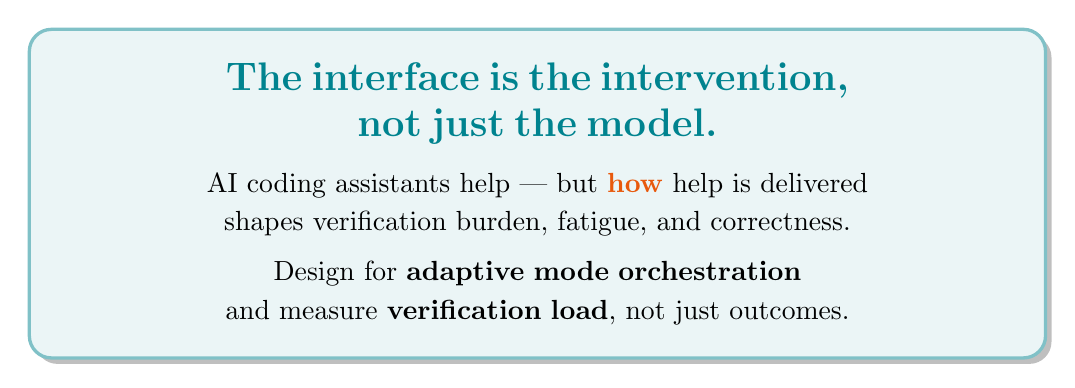
\begin{tikzpicture}
  \node[rounded corners=8pt, fill=chiTeal!8, draw=chiTeal!50, line width=1.2pt,
    inner xsep=20pt, inner ysep=12pt, text width=11.5cm, align=center,
    drop shadow] {
    {\Large\bfseries\textcolor{chiTeal}{The interface is the intervention,}}\\[3pt]
    {\Large\bfseries\textcolor{chiTeal}{not just the model.}}\\[8pt]
    {\normalsize
    AI coding assistants help --- but \emphmark{how} help is delivered\\[2pt]
    shapes verification burden, fatigue, and correctness.\\[6pt]
    Design for \textbf{adaptive mode orchestration}\\[2pt]
    and measure \textbf{verification load}, not just outcomes.}
  };
\end{tikzpicture}
\end{center}
\vspace{1pt}
\begin{columns}[T]
\begin{column}{0.32\textwidth}
\begin{findingbox}
\scriptsize \textbf{AI vs.\ Control:}\\
$-18.2$ TLX \textbullet{} 22\% faster\\
OR $= 1.71$ correctness
\end{findingbox}
\end{column}
\begin{column}{0.32\textwidth}
\begin{findingbox}
\scriptsize \textbf{$V_{\text{core}}$ mediates:}\\
$\sim$26\% fatigue\\
$\sim$24\% stress
\end{findingbox}
\end{column}
\begin{column}{0.32\textwidth}
\begin{findingbox}
\scriptsize \textbf{Crossover:}\\
Chat $>$ Inline at $z{>}+0.41$\\
Accept sweet spot $\approx$48\%
\end{findingbox}
\end{column}
\end{columns}
\vspace{4pt}
\begin{center}
{\scriptsize \textcolor{chiGray}{Guangrui Fan ~~\textbullet~~ fgr@tyust.edu.cn
 ~~\textbullet~~ DOI: \texttt{10.1145/3772318.3791176}}}
\end{center}
\end{frame}

% ============================================================
%  THANK YOU
% ============================================================
{
\setbeamertemplate{footline}{}
\begin{frame}[plain,noframenumbering]
\begin{tikzpicture}[remember picture, overlay]
  \fill[chiDeep] (current page.north west) rectangle (current page.south east);
  \mosaicCorner{-6.5}{3.5}{2.0}
  \mosaicCorner{5.0}{3.0}{1.6}
  \mosaicCorner{-5.5}{-3.0}{1.4}
  \mosaicCorner{6.0}{-3.5}{1.8}
  \node[text=white, font=\Huge\bfseries] at ([yshift=12mm]current page.center)
    {Thank You!};
  \node[text=white!80, font=\large] at ([yshift=-2mm]current page.center)
    {Questions \& Discussion};
  \node[text=white!70, font=\small, text width=10cm, align=center]
    at ([yshift=-18mm]current page.center) {
    \faEnvelope~~fgr@tyust.edu.cn \qquad
    \faFile*~~DOI: 10.1145/3772318.3791176};
  \fill[white, opacity=0.92]
    ([yshift=0mm]current page.south west) rectangle
    ([yshift=16mm]current page.south east);
  \node[anchor=south west] at ([xshift=14mm, yshift=2mm]current page.south west)
    {
\includegraphics[height=1.1cm]{assets/tyust-logo.png}};
  \node[anchor=south] at ([xshift=-20mm, yshift=2.5mm]current page.south)
    {
\includegraphics[height=1.0cm]{assets/chi2026-logo.png}};
  \node[anchor=south] at ([xshift=20mm, yshift=2mm]current page.south)
    {
\includegraphics[height=1.0cm]{assets/acm-logo.png}};
  \node[anchor=south east] at ([xshift=-14mm, yshift=3mm]current page.south east)
    {
\includegraphics[height=0.9cm]{assets/sigchi-logo.png}};
\end{tikzpicture}
\end{frame}
}

\end{document}
